%% Thesis language: english or polish
%% Thesis type: master or engineer
\documentclass[polish,engineer]{polsl-msth}
%% set document encoding
\usepackage[utf8]{inputenc}

%% other packages
\usepackage{tikz}
\usepackage{gensymb}
\usepackage{pstricks}
\usepackage{hyperref}

%% thesis author
\author{Michał Dobrut}

%% thesis supervisor
\supervisor{dr Krzysztof Mazur}

%% thesis consultant, optional
%% \consultant{Jan Kowalski}

%% Thesis title
\title{Mikroprocesorowa ładowarka ogniw litowo-jonowych}
\begin{document}
\frontmatter
\maketitle
\makestatement
\tableofcontents
\listoftables
\listoffigures
\mainmatter

\usepackage{color}
\definecolor{GREEN}{rgb}{0,0.5,0}
\newcommand{\remark}[1]{{[\color{GREEN}\emph{\footnotesize #1}{}]}}

\chapter{Wprowadzenie}

Współcześnie ogniwa litowo-jonowe zdominowały rynek przechowywania energii dla urządzeń przenośnych oraz pojazdów\remark{elektrycznych i~hybrydowych? bo w spalinowych raczej dominują nadal ołowiowe}. W związku z tym od 20 lat można obserwować intensywne badania mające na celu poprawę parametrów ogniw i testowanie nowych technologii. Spadająca cena i poprawa właściwości powoduje wzrost zapotrzebowania, zwłaszcza za sprawą popularyzacji samochodów osobowych z napędem elektrycznym (EV). Branża automotive stawia bardzo wysokie wymagania dla akumulatorów samochodów EV: wymagana jest duża gęstość energetyczna, wysoka szybkość ładowania i ponadprzeciętna trwałość. Wciąż badane są nowe strategie ładowania które pozwalały by zachować wysokie parametry przy minimalizacji czasu ładowania.

Niniejszy projekt inżynierski wpisuje się w ten trend, proponując ładowarkę pozwalającą z dużą elastycznością kształtować przebieg procesu ładowania. Docelowo urządzenie to ma umożliwiać przeprowadzenie ograniczonych badań wpływu sposobu ładowania na parametry ogniwa. Z uwagi na dominującą pozycję na rynku ogniw w standardzie 18650, taki rozmiar został wybrany za docelowy. 

W projekcie położony jest nacisk na stworzenie regulatora, pozwalającego realizować założone przebiegi napięcia i prądu na ogniwie. Zadanie nastawiania prądu jest zrealizowane za pomocą tranzystora MOSFET\remark{część FET jest chyba bardziej ostotna jak MOS}, pracującego w zakresie triodowym, którego otwieraniem steruje wzmacniacz operacyjny, tworząc źródło prądowe. Nad napięciem na ogniwie czuwa regulator PI, który tak steruje prądem, aby utrzymać je w założonym przedziale\remark{sam PI to raczej pojedynczej wartości zadanej}. Nad całością operacji kontrolę sprawuje skrypt w środowisku MATLAB, który odpowiada za wypracowywanie sygnału sterującego prądem oraz zbieranie i wyświetlanie danych z procesu.

W trakcie prac użyte zostały 2 modele ogniwa. Podczas projektowania części sprzętowej wykorzystano model Thevenina 1. rzędu, a podczas dobierania nastaw regulatora wykorzystywano transmitancję operatorową, której parametry pobrano badając obiekt rzeczywisty. 

\remark{Nie wiem, czy nie ma tu za dużo ,,jak'', a zamało ,,po co''.}

\chapter{Teoria}
\section{Budowa i specyfika działania ogniw litowo-jonowych}
Historia użytecznych ogniw na bazie litu sięga lat 70, kiedy Adam Heller opatentował pierwszą kompozycję chemiczną anody, katody i elektrolitu \cite{heller1975electrochemical}, pozwalającą na skonstruowanie baterii w cenach akceptowalnych przez rynek. Od tego czasu dostępnych jest wiele technologii wykonania takich ogniw, różniących się ze względu na wykorzystane materiały. Zasadę działania obecnie już wycofywanej technologii przedstawia\remark{to, że technologia jest wycofana raczej nie powinno być jej opisem, np. działania popularnej kiedyś techologii, ale obecnie wycofanej, albo cokolwiek mówiący w pozytywny sposób o tej technologii, bo przy negatywnym opisywaniu czegoś to trzeba podać mnóstwo rzeczy czymś to nie jest} rys. \ref{img:liion_structure}.
\begin{figure}[hbtp]
\centering
     \resizebox{0.45\linewidth}{!}{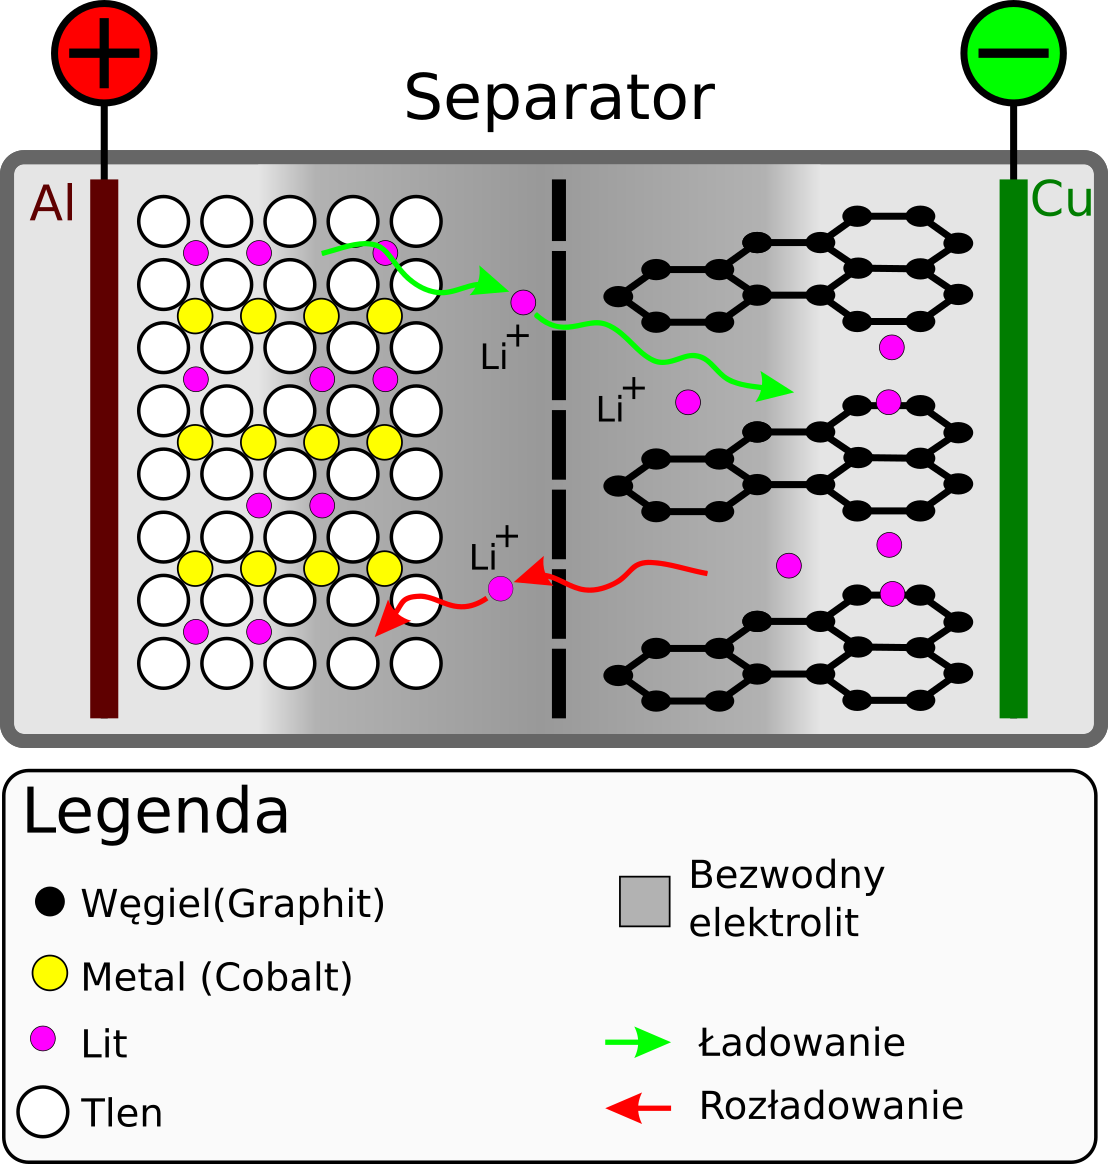
\includegraphics[]{img/liion_structure.png}}
     \caption{Budowa i działanie ogniwa z anodą grafitową i katodą LCO. \cite{liionpic_wikimedia}  \label{img:liion_structure}}
\end{figure}
Na tle innych technologii akumulatory litowo-jonowe przodują zarówno pod wpływem wagowej gęstości energetycznej jak i wagowej gęstości mocy. I główną wadą jest jednak trwałość w warunkach powtarzającego wykorzystywania pełnej pojemności. \cite{IBRAHIM20081221} Jest to powód, dla którego ogniwa te znalazły zastosowanie głównie w urządzeniach przenośnych i pojazdach oraz systemach awaryjnego zasilania, a w mniejszym stopniu do wyrównywania mocy dostarczanej do sieci elektrycznej.

\remark{brakuje mi trochę tutaj powiedzenia dlaczego akurat lit, a z tego
co kojarzę to chodzi o jego małą masę, dużą reaktywność, dużo elektronów
walencyjnych w stosunku do masy.}

\section{Porównanie chemii}
Obecnie dominującą rolę przejęły ogniwa oparte o katodę niklowo-manganowo-kobaltową NMC (w różnych proporcjach składników, dąży się do wyeliminowania lub zmniejszenia udziału drogiego kobaltu) oraz niklowo-kobaltowo-aluminiową NCA.\cite{bu_liiontypes} W zastosowaniach wymagających dużego bezpieczeństwa i długiej żywotności używa się także katod z fosforanu litowo-żelazowego LFP lub anod z tytanku litu LTO. Pozostałe technologie wychodzą z użytku, są bardzo drogie lub na razie mają wąski zakres zastosowań. W tabeli \ref{tab:chemisties_voltages} zebrano parametry interesujące ze względu na konstrukcję ładowarki.
\begin{table}[hbtp]
\caption{Wybrane parametry zależne od technologii ogniwa.\cite{bu_liiontypes} \label{tab:chemisties_voltages}}
\centerline{\begin{tabular}{|c|c|c|c|c|}
\hline
Technologia & Napięcie maks., V & Napięcie min., V & Szybkość ład., C & Żywotność, cykle \\
\hline
LCO & 4.2 & 2.5 & 0.7--1 & 500--1000\\
\hline
LMO & 4.2 & 2.5 & 0.7--1 & 300--700\\
\hline 
NMC & 4.2 & 2.5 & 0.7--1 & 1000--2000\\ \hline
LFP & 3.65 & 2.5 & 1 & 2000+\\ \hline
NCA & 4.2 & 3.0 & 0.7 & 500\\ \hline
LTO & 2.85 & 1.8 & 1 & 3000--7000\\ \hline
\end{tabular}}
\end{table}
\remark{przy zakresach powinno być `-{}-'}

Ładowarka była projektowana dla najpopularniejszych ogniw na rynku, jednak dzięki odpowiednio dobranym komponentom jest w stanie działać także dla ogniw w technologii LTO, z ograniczeniem prądu ładowania.

\section{Strategie ładowania}
Ogniwa litowo jonowe, w większości przypadków optymalizowane aby osiągnąć maksymalną gęstość energetyczną, wykazują dużą wrażliwość na przekroczenie ograniczeń prądowych ładowania\cite{TOMASZEWSKA2019100011}, które w dobie rozwoju samochodów elektrycznych są czynnikiem mocno ograniczającym szeroką popularyzację. W związku z tym, badane są rozmaite strategie ładowania. Odpowiedni dobór profilu prądowego pozwala na podwojenie żywotności baterii w stosunku do ładowania profilem CC-CV, przy czasie ładowania dłuższym o około 15\%\cite{SCHINDLER2018364}.
\begin{figure}[hbtp]
     \resizebox{\linewidth}{!}{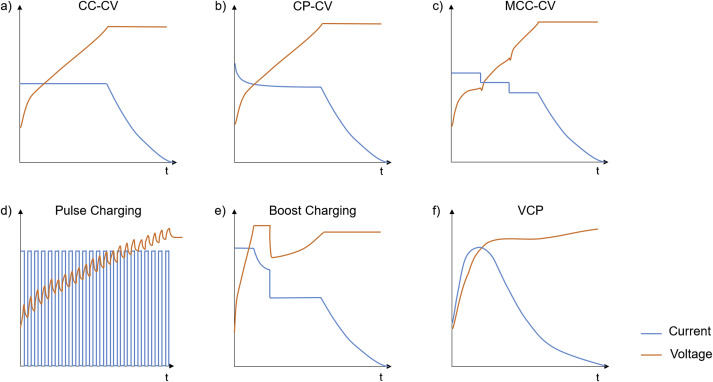
\includegraphics[]{img/protocols.jpg}}
     \caption{Różne strategie ładowania \cite{TOMASZEWSKA2019100011}.\label{img:charging_protocols}}
\end{figure}

Najbardziej rozpowszechnionym i rekomendowanym przez producentów schematem ładowania jest CC-CV, czyli utrzymywanie stałego prądu do momentu osiągnięcia zadanego napięcia maksymalnego, potem utrzymywanie tego napięcia, aż prąd spadnie poniżej zadanej wartości.

Jeżeli zaimplementowane zostaną metody programowej kontroli tych parametrów, możliwe jest także wykorzystanie dowolnego innego protokołu, tak długo jak jego wymagania prądowe i napięciowe mogą być spełnione przez ładowarkę.

\section{Model matematyczny ogniwa}
Powstało wiele dokładnych modeli\cite{1634598_BATT_MODELS} ogniw litowo-jonowych, modelujących stan naładowania i odpowiedzi czasowe z dokładnością poniżej 1\%, jednak na potrzeby weryfikacji jakości regulacji prądu na poziomie sprzętowym, ze względu na małą dynamikę zmian, użyty został zastępczy model elektryczny 1. rzędu o parametrach jak w \cite{8759769_cellmodel1storder} (rys. \ref{img:thevenin_model}). Dzięki niemu możliwe było prowadzenie symulacji zachowania się układu w LTSpice.
\begin{figure}[hbtp]
    \centering
     \resizebox{0.5\linewidth}{!}{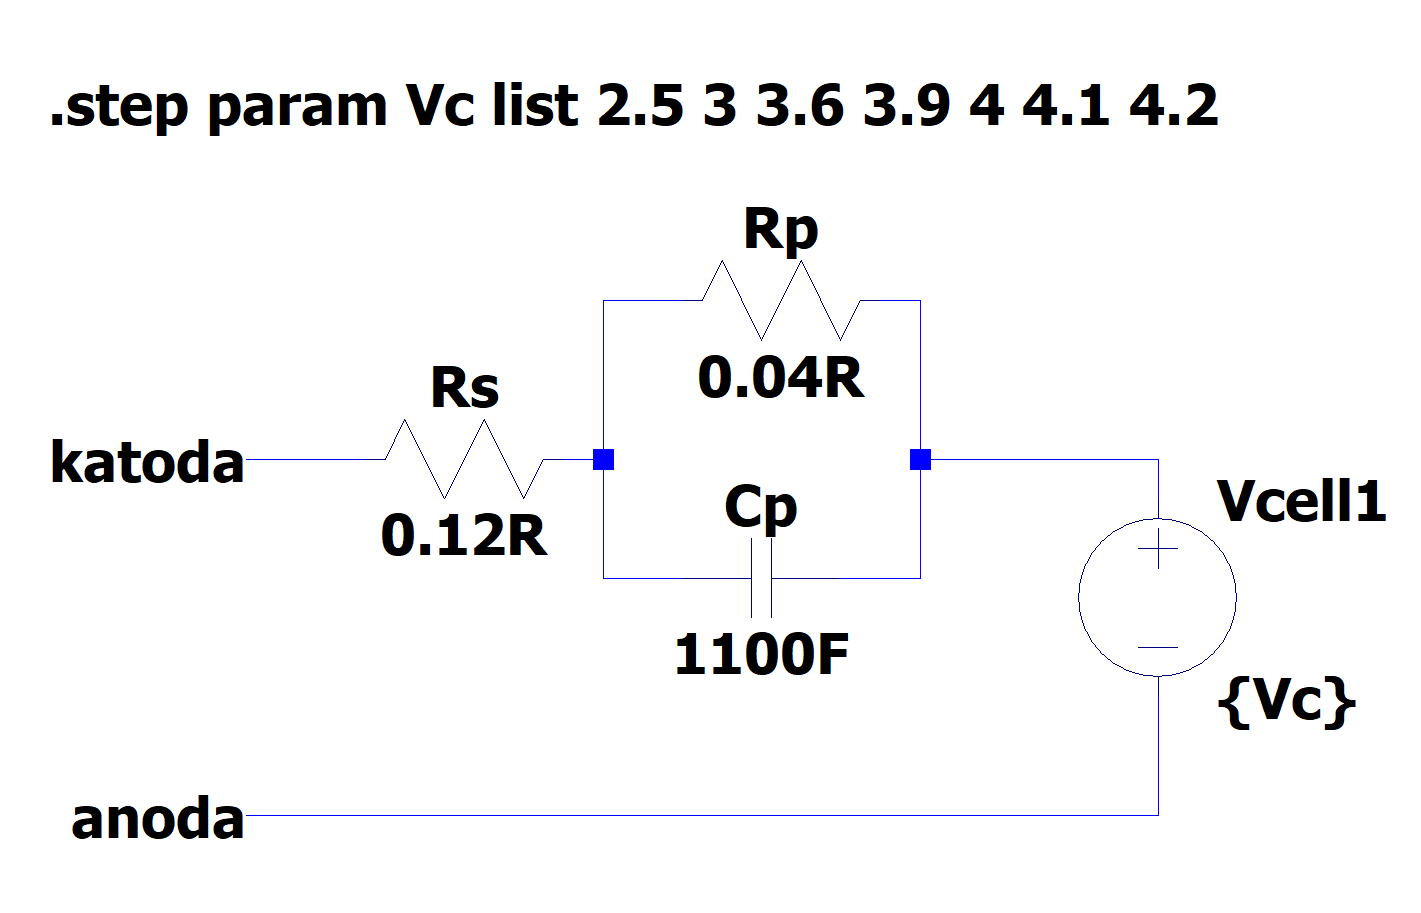
\includegraphics[]{img/cell_model.png}}
     \caption{Model elektryczny ogniwa.\label{img:thevenin_model}}
\end{figure}

W celu znalezienia zadowalających nastaw regulatora napięcia, na podstawie charakteru odpowiedzi układu określono jego przybliżony model. Obserwacja kształtu odpowiedzi na skokową zmianę parametrów pozwoliła na stwierdzenie struktury transmitancji (równanie \ref{eq:transmit_modelu}). Znaczną 'pojemność', w sensie analogu elektrycznego ogniwa, odpowiadającą za powolny wzrost napięcia podczas ładowania, przybliżono za pomocą całki.
\begin{equation}
    K(s) = k\frac{s\tau_1 + 1}{s(s\tau_2 + 1)}
    \label{eq:transmit_modelu}
\end{equation}
Parametry transmitancji znaleziono za pomocą MATLAB Model Identification Toolbox.

\remark{tutaj trochę czegoś nie rozumiem, podaje Pan wcześniej model ogniwa,
a później pisze Pan o tym, że obserwacja kształtu odpowiedzi skokowej pozwoliła na stwierdzenie struktury transmitacji. I też ta transmitacja nie pasuje do tego modelu powyżej.}

\section{Regulator}
Aby realizować wybraną strategię, konieczne jest użycie struktury regulatora zapewniającej stabilne działanie nawet przy pewnej zmienności parametrów obiektu, wynikającej z różnic technologicznych pomiędzy ogniwami. Wymagania te spełnia, przy jednoczesnym zachowaniu łatwości implementacji, regulator PI.
\begin{equation}
     u(t)=k_{p}\left[e(t)+{\frac {1}{T_{i}}}\int _{0}^{t}e(\tau )d\tau \right]
     \label{eq:PI_timebased}
\end{equation}
Ze względu na częstotliwość próbkowania znacznie większa od stałych czasowych procesu wykorzystano możliwość analizy regulatora jako układu ciągłego.\remark{to niestety nie jest do końca prawdą, choć znam pewnie źródło, pewna osoba, która może tego do końca nie rozumie. Jak ma Pan skrypt prof. Gessinga to dobrze sobie tam o tym poczytać.}

Strategie ładowania zakładają możliwość utrzymywania zadanego prądu (regulator sprzętowy) lub zadanego napięcia (regulator programowy), dlatego konieczne jest zapewnienie bezuderzeniowego przełączania między trybami. Jest to realizowane przez ciągłe wyliczanie odpowiedniej wartości całki podczas trybu stabilizacji prądu. Jednocześnie wartość procesowa jaką jest zadany prąd jest wspólna dla obu trybów.

\remark{a to mnie trochę zdziwiło, ja spodziewałem się prostego ukłądu kaskadowego,
gdzie regulator napięcia ma po prostu stała wartość zadaną przy ładowaniu
CC-CV, i przez część CC to po prostu działa na ograniczeniu sterowania.}

\chapter{Projekt urządzenia}
\section{Założenia}
Urządzenie ma być zdolne do ładowania ogniw litowo-jonowych o różnym składzie anody i katody w standardzie wymiarowym 18650 z ciągłym prądem maksymalnym 3~A. Prąd ładowania ma być regulowany z rozdzielczością powyżej 20~mA, a napięcie utrzymywane z dokładnością do 20~mV. Urządzenie jest zasilane z zasilacza impulsowego o napięciu 5~V i odpowiedniej mocy.\remark{według ISO-31 powinna być spacja pomiędzy wartością,
a jednostką}
\section{Identyfikacja kluczowych obszarów projektu}
Aby można było realizować płynną regulację prądu wyjściowego można zastosować regulator liniowy lub przetwornice impulsowa o regulowanym napięciu wyjściowym. Ze względu na fakt, że urządzenie ma nadawać się do badań wpływu procesu ładowania na parametry ogniw, zdecydowano się na regulator liniowy, aby nie trzeba było badać stabilności napięcia ładowania i poziomu\remark{wielkości szumu? wielkość musi dotyczyć jakiejś miary.} niepożądanych szumów, mogących wpłynąć na jakość wyników prób. Wybrany sposób ograniczenia prądu ma taką zaletę, że tłumi zakłócenia pochodzące z zasilania.

Wadą tego rozwiązania jest spora strata energii, a w konsekwencji znaczące wydzielanie się ciepła w układzie. Dla układu tworzonego w celach badawczych takie marnotrawstwo energii jest bez znaczenia, jednak temperatura komponentów ma duży wpływ na ich żywotność, a co za tym idzie powtarzalność procesu. Stąd istotne dla stabilnego działania układu jest zapewnienie skutecznego chłodzenia.

Aby można było śledzić postęp ładowania i w prosty sposób zadawać parametry, przydatna jest komunikacja z komputerem. Wymagania co do kanału komunikacyjnego nie są wygórowane --- ilość danych do przekazania jest niewielka, a okres przesyłania jest rzędu 1s.

Kontroler układu musi odpowiadać także za kwestie bezpieczeństwa --- minimalna funkcjonalność to ograniczenie lub odcięcie prądu w przypadku wzrostu temperatury ogniwa ponad ustaloną wartość.

\section{Proponowane rozwiązania i wybór komponentów}
Ze względu na wysoki założony prąd ładowania i niewielką różnicę napięcia pomiędzy maksymalnym napięciem na ogniwie (4.2V) a napięciem zasilania (5V) nie znaleziono żadnych gotowych rozwiązań zintegrowanych pozwalających na dostatecznie precyzyjną kontrolę prądu. W związku z tym wybrano rozwiązanie oparte o tranzystor MOSFET z kanałem typu P, sterowny przez wzmacniacz operacyjny w pętli sprzężenia zwrotnego.

Podczas działania układu, w momencie gdy ogniwo jest rozładowane, a napięcie na nim wynosi 3V, dla prądu maksymalnego moc wydzielana na tranzystorze wynosi $5.3\mathrm{W}$. Jest to stosunkowo dużo, zważywszy na małe rozmiary współczesnych tranzystorów spełniających wysokie wymagania\remark{te wysokie wymagania są też nie jasne, czy napięcie graniczne ma być małe, czy duże?} dotyczące napięcie granicznego otwarcia. W tym celu użyto laminatu o ponadstandardowej grubości miedzi \remark{jak rozumiem to chodzi o grubość miedzi, a nie dielektryka, który im grubszy tym gorzej.} i pasywnych radiatorów wlutowanych bezpośrednio wokół tranzystora.

Do sterowania całym układem wybrano 8-bitowy mikrokontroler firmy Microchip: ATtiny414. Zawiera on wszystkie potrzebne peryferia od razu zintegrowane w jednym układzie, przy jednoczesnym zachowaniu niskiej ceny. 
\section{Projekt struktury}
Wybrana struktura układu regulacji prezentuje się jak na rys. \ref{dia:reg_all}. 
\begin{figure}
     \resizebox{\linewidth}{!}{% Graphic for TeX using PGF
% Title: /home/dobi/transfer/inz/charger-v2/dia/control_flow.dia
% Creator: Dia v0.97+git
% CreationDate: Wed Jan  8 12:19:36 2020
% For: dobi
% \usepackage{tikz}
% The following commands are not supported in PSTricks at present
% We define them conditionally, so when they are implemented,
% this pgf file will use them.
\ifx\du\undefined
  \newlength{\du}
\fi
\setlength{\du}{15\unitlength}
\begin{tikzpicture}[even odd rule]
\pgftransformxscale{1.000000}
\pgftransformyscale{-1.000000}
\definecolor{dialinecolor}{rgb}{0.000000, 0.000000, 0.000000}
\pgfsetstrokecolor{dialinecolor}
\pgfsetstrokeopacity{1.000000}
\definecolor{diafillcolor}{rgb}{1.000000, 1.000000, 1.000000}
\pgfsetfillcolor{diafillcolor}
\pgfsetfillopacity{1.000000}
\pgfsetlinewidth{0.100000\du}
\pgfsetdash{}{0pt}
\pgfsetmiterjoin
{\pgfsetcornersarced{\pgfpoint{0.000000\du}{0.000000\du}}\definecolor{diafillcolor}{rgb}{1.000000, 1.000000, 1.000000}
\pgfsetfillcolor{diafillcolor}
\pgfsetfillopacity{1.000000}
\fill (20.000000\du,14.000000\du)--(20.000000\du,21.000000\du)--(30.000000\du,21.000000\du)--(30.000000\du,14.000000\du)--cycle;
}{\pgfsetcornersarced{\pgfpoint{0.000000\du}{0.000000\du}}\definecolor{dialinecolor}{rgb}{0.000000, 0.000000, 0.000000}
\pgfsetstrokecolor{dialinecolor}
\pgfsetstrokeopacity{1.000000}
\draw (20.000000\du,14.000000\du)--(20.000000\du,21.000000\du)--(30.000000\du,21.000000\du)--(30.000000\du,14.000000\du)--cycle;
}% setfont left to latex
\definecolor{dialinecolor}{rgb}{0.000000, 0.000000, 0.000000}
\pgfsetstrokecolor{dialinecolor}
\pgfsetstrokeopacity{1.000000}
\definecolor{diafillcolor}{rgb}{0.000000, 0.000000, 0.000000}
\pgfsetfillcolor{diafillcolor}
\pgfsetfillopacity{1.000000}
\node[anchor=base,inner sep=0pt, outer sep=0pt,color=dialinecolor] at (25.000000\du,17.695000\du){};
% setfont left to latex
\definecolor{dialinecolor}{rgb}{0.000000, 0.000000, 0.000000}
\pgfsetstrokecolor{dialinecolor}
\pgfsetstrokeopacity{1.000000}
\definecolor{diafillcolor}{rgb}{0.000000, 0.000000, 0.000000}
\pgfsetfillcolor{diafillcolor}
\pgfsetfillopacity{1.000000}
\node[anchor=base west,inner sep=0pt,outer sep=0pt,color=dialinecolor] at (17.700000\du,16.750000\du){Uset};
% setfont left to latex
\definecolor{dialinecolor}{rgb}{0.000000, 0.000000, 0.000000}
\pgfsetstrokecolor{dialinecolor}
\pgfsetstrokeopacity{1.000000}
\definecolor{diafillcolor}{rgb}{0.000000, 0.000000, 0.000000}
\pgfsetfillcolor{diafillcolor}
\pgfsetfillopacity{1.000000}
\node[anchor=base west,inner sep=0pt,outer sep=0pt,color=dialinecolor] at (17.700000\du,17.550000\du){};
% setfont left to latex
\definecolor{dialinecolor}{rgb}{0.000000, 0.000000, 0.000000}
\pgfsetstrokecolor{dialinecolor}
\pgfsetstrokeopacity{1.000000}
\definecolor{diafillcolor}{rgb}{0.000000, 0.000000, 0.000000}
\pgfsetfillcolor{diafillcolor}
\pgfsetfillopacity{1.000000}
\node[anchor=base west,inner sep=0pt,outer sep=0pt,color=dialinecolor] at (30.350000\du,16.700000\du){Ug};
% setfont left to latex
\definecolor{dialinecolor}{rgb}{0.000000, 0.000000, 0.000000}
\pgfsetstrokecolor{dialinecolor}
\pgfsetstrokeopacity{1.000000}
\definecolor{diafillcolor}{rgb}{0.000000, 0.000000, 0.000000}
\pgfsetfillcolor{diafillcolor}
\pgfsetfillopacity{1.000000}
\node[anchor=base west,inner sep=0pt,outer sep=0pt,color=dialinecolor] at (38.600000\du,16.700000\du){I};
% setfont left to latex
\definecolor{dialinecolor}{rgb}{0.000000, 0.000000, 0.000000}
\pgfsetstrokecolor{dialinecolor}
\pgfsetstrokeopacity{1.000000}
\definecolor{diafillcolor}{rgb}{0.000000, 0.000000, 0.000000}
\pgfsetfillcolor{diafillcolor}
\pgfsetfillopacity{1.000000}
\node[anchor=base west,inner sep=0pt,outer sep=0pt,color=dialinecolor] at (48.350000\du,16.700000\du){Ucell};
\pgfsetlinewidth{0.100000\du}
\pgfsetdash{}{0pt}
\pgfsetmiterjoin
{\pgfsetcornersarced{\pgfpoint{0.000000\du}{0.000000\du}}\definecolor{diafillcolor}{rgb}{1.000000, 1.000000, 1.000000}
\pgfsetfillcolor{diafillcolor}
\pgfsetfillopacity{1.000000}
\fill (10.000000\du,15.000000\du)--(10.000000\du,19.000000\du)--(17.000000\du,19.000000\du)--(17.000000\du,15.000000\du)--cycle;
}{\pgfsetcornersarced{\pgfpoint{0.000000\du}{0.000000\du}}\definecolor{dialinecolor}{rgb}{0.000000, 0.000000, 0.000000}
\pgfsetstrokecolor{dialinecolor}
\pgfsetstrokeopacity{1.000000}
\draw (10.000000\du,15.000000\du)--(10.000000\du,19.000000\du)--(17.000000\du,19.000000\du)--(17.000000\du,15.000000\du)--cycle;
}% setfont left to latex
\definecolor{dialinecolor}{rgb}{0.000000, 0.000000, 0.000000}
\pgfsetstrokecolor{dialinecolor}
\pgfsetstrokeopacity{1.000000}
\definecolor{diafillcolor}{rgb}{0.000000, 0.000000, 0.000000}
\pgfsetfillcolor{diafillcolor}
\pgfsetfillopacity{1.000000}
\node[anchor=base,inner sep=0pt, outer sep=0pt,color=dialinecolor] at (13.500000\du,16.795000\du){uC};
% setfont left to latex
\definecolor{dialinecolor}{rgb}{0.000000, 0.000000, 0.000000}
\pgfsetstrokecolor{dialinecolor}
\pgfsetstrokeopacity{1.000000}
\definecolor{diafillcolor}{rgb}{0.000000, 0.000000, 0.000000}
\pgfsetfillcolor{diafillcolor}
\pgfsetfillopacity{1.000000}
\node[anchor=base,inner sep=0pt, outer sep=0pt,color=dialinecolor] at (13.500000\du,17.595000\du){Uset(Ucell)};
\pgfsetlinewidth{0.100000\du}
\pgfsetdash{}{0pt}
\pgfsetmiterjoin
{\pgfsetcornersarced{\pgfpoint{0.000000\du}{0.000000\du}}\definecolor{diafillcolor}{rgb}{1.000000, 1.000000, 1.000000}
\pgfsetfillcolor{diafillcolor}
\pgfsetfillopacity{1.000000}
\fill (25.000000\du,15.000000\du)--(25.000000\du,19.000000\du)--(29.000000\du,19.000000\du)--(29.000000\du,15.000000\du)--cycle;
}{\pgfsetcornersarced{\pgfpoint{0.000000\du}{0.000000\du}}\definecolor{dialinecolor}{rgb}{0.000000, 0.000000, 0.000000}
\pgfsetstrokecolor{dialinecolor}
\pgfsetstrokeopacity{1.000000}
\draw (25.000000\du,15.000000\du)--(25.000000\du,19.000000\du)--(29.000000\du,19.000000\du)--(29.000000\du,15.000000\du)--cycle;
}% setfont left to latex
\definecolor{dialinecolor}{rgb}{0.000000, 0.000000, 0.000000}
\pgfsetstrokecolor{dialinecolor}
\pgfsetstrokeopacity{1.000000}
\definecolor{diafillcolor}{rgb}{0.000000, 0.000000, 0.000000}
\pgfsetfillcolor{diafillcolor}
\pgfsetfillopacity{1.000000}
\node[anchor=base,inner sep=0pt, outer sep=0pt,color=dialinecolor] at (27.000000\du,17.195000\du){-k};
\pgfsetlinewidth{0.100000\du}
\pgfsetdash{}{0pt}
\pgfsetbuttcap
\pgfsetmiterjoin
\pgfsetlinewidth{0.100000\du}
\pgfsetbuttcap
\pgfsetmiterjoin
\pgfsetdash{}{0pt}
\definecolor{diafillcolor}{rgb}{1.000000, 1.000000, 1.000000}
\pgfsetfillcolor{diafillcolor}
\pgfsetfillopacity{1.000000}
\pgfpathellipse{\pgfpoint{23.000000\du}{17.000000\du}}{\pgfpoint{1.000000\du}{0\du}}{\pgfpoint{0\du}{1.000000\du}}
\pgfusepath{fill}
\definecolor{dialinecolor}{rgb}{0.000000, 0.000000, 0.000000}
\pgfsetstrokecolor{dialinecolor}
\pgfsetstrokeopacity{1.000000}
\pgfpathellipse{\pgfpoint{23.000000\du}{17.000000\du}}{\pgfpoint{1.000000\du}{0\du}}{\pgfpoint{0\du}{1.000000\du}}
\pgfusepath{stroke}
\pgfsetbuttcap
\pgfsetmiterjoin
\pgfsetdash{}{0pt}
\definecolor{dialinecolor}{rgb}{0.000000, 0.000000, 0.000000}
\pgfsetstrokecolor{dialinecolor}
\pgfsetstrokeopacity{1.000000}
\draw (22.292900\du,16.292900\du)--(23.707100\du,17.707100\du);
\pgfsetbuttcap
\pgfsetmiterjoin
\pgfsetdash{}{0pt}
\definecolor{dialinecolor}{rgb}{0.000000, 0.000000, 0.000000}
\pgfsetstrokecolor{dialinecolor}
\pgfsetstrokeopacity{1.000000}
\draw (22.292900\du,17.707100\du)--(23.707100\du,16.292900\du);
\pgfsetlinewidth{0.100000\du}
\pgfsetdash{}{0pt}
\pgfsetbuttcap
{
\definecolor{diafillcolor}{rgb}{0.000000, 0.000000, 0.000000}
\pgfsetfillcolor{diafillcolor}
\pgfsetfillopacity{1.000000}
% was here!!!
\pgfsetarrowsend{stealth}
\definecolor{dialinecolor}{rgb}{0.000000, 0.000000, 0.000000}
\pgfsetstrokecolor{dialinecolor}
\pgfsetstrokeopacity{1.000000}
\draw (17.000000\du,17.000000\du)--(22.000000\du,17.000000\du);
}
\pgfsetlinewidth{0.100000\du}
\pgfsetdash{}{0pt}
\pgfsetbuttcap
{
\definecolor{diafillcolor}{rgb}{0.000000, 0.000000, 0.000000}
\pgfsetfillcolor{diafillcolor}
\pgfsetfillopacity{1.000000}
% was here!!!
\pgfsetarrowsend{stealth}
\definecolor{dialinecolor}{rgb}{0.000000, 0.000000, 0.000000}
\pgfsetstrokecolor{dialinecolor}
\pgfsetstrokeopacity{1.000000}
\draw (24.000000\du,17.000000\du)--(25.000000\du,17.000000\du);
}
\pgfsetlinewidth{0.100000\du}
\pgfsetdash{}{0pt}
\pgfsetmiterjoin
{\pgfsetcornersarced{\pgfpoint{0.000000\du}{0.000000\du}}\definecolor{diafillcolor}{rgb}{1.000000, 1.000000, 1.000000}
\pgfsetfillcolor{diafillcolor}
\pgfsetfillopacity{1.000000}
\fill (32.000000\du,15.000000\du)--(32.000000\du,19.000000\du)--(38.000000\du,19.000000\du)--(38.000000\du,15.000000\du)--cycle;
}{\pgfsetcornersarced{\pgfpoint{0.000000\du}{0.000000\du}}\definecolor{dialinecolor}{rgb}{0.000000, 0.000000, 0.000000}
\pgfsetstrokecolor{dialinecolor}
\pgfsetstrokeopacity{1.000000}
\draw (32.000000\du,15.000000\du)--(32.000000\du,19.000000\du)--(38.000000\du,19.000000\du)--(38.000000\du,15.000000\du)--cycle;
}% setfont left to latex
\definecolor{dialinecolor}{rgb}{0.000000, 0.000000, 0.000000}
\pgfsetstrokecolor{dialinecolor}
\pgfsetstrokeopacity{1.000000}
\definecolor{diafillcolor}{rgb}{0.000000, 0.000000, 0.000000}
\pgfsetfillcolor{diafillcolor}
\pgfsetfillopacity{1.000000}
\node[anchor=base,inner sep=0pt, outer sep=0pt,color=dialinecolor] at (35.000000\du,17.195000\du){MOSFET};
\pgfsetlinewidth{0.100000\du}
\pgfsetdash{}{0pt}
\pgfsetmiterjoin
{\pgfsetcornersarced{\pgfpoint{0.000000\du}{0.000000\du}}\definecolor{diafillcolor}{rgb}{1.000000, 1.000000, 1.000000}
\pgfsetfillcolor{diafillcolor}
\pgfsetfillopacity{1.000000}
\fill (41.000000\du,15.000000\du)--(41.000000\du,19.000000\du)--(48.000000\du,19.000000\du)--(48.000000\du,15.000000\du)--cycle;
}{\pgfsetcornersarced{\pgfpoint{0.000000\du}{0.000000\du}}\definecolor{dialinecolor}{rgb}{0.000000, 0.000000, 0.000000}
\pgfsetstrokecolor{dialinecolor}
\pgfsetstrokeopacity{1.000000}
\draw (41.000000\du,15.000000\du)--(41.000000\du,19.000000\du)--(48.000000\du,19.000000\du)--(48.000000\du,15.000000\du)--cycle;
}% setfont left to latex
\definecolor{dialinecolor}{rgb}{0.000000, 0.000000, 0.000000}
\pgfsetstrokecolor{dialinecolor}
\pgfsetstrokeopacity{1.000000}
\definecolor{diafillcolor}{rgb}{0.000000, 0.000000, 0.000000}
\pgfsetfillcolor{diafillcolor}
\pgfsetfillopacity{1.000000}
\node[anchor=base,inner sep=0pt, outer sep=0pt,color=dialinecolor] at (44.500000\du,16.795000\du){Ogniwo};
% setfont left to latex
\definecolor{dialinecolor}{rgb}{0.000000, 0.000000, 0.000000}
\pgfsetstrokecolor{dialinecolor}
\pgfsetstrokeopacity{1.000000}
\definecolor{diafillcolor}{rgb}{0.000000, 0.000000, 0.000000}
\pgfsetfillcolor{diafillcolor}
\pgfsetfillopacity{1.000000}
\node[anchor=base,inner sep=0pt, outer sep=0pt,color=dialinecolor] at (44.500000\du,17.595000\du){Ucell(I, SOC, To)};
\pgfsetlinewidth{0.100000\du}
\pgfsetdash{}{0pt}
\pgfsetmiterjoin
{\pgfsetcornersarced{\pgfpoint{0.000000\du}{0.000000\du}}\definecolor{diafillcolor}{rgb}{1.000000, 1.000000, 1.000000}
\pgfsetfillcolor{diafillcolor}
\pgfsetfillopacity{1.000000}
\fill (32.000000\du,21.000000\du)--(32.000000\du,25.000000\du)--(36.000000\du,25.000000\du)--(36.000000\du,21.000000\du)--cycle;
}{\pgfsetcornersarced{\pgfpoint{0.000000\du}{0.000000\du}}\definecolor{dialinecolor}{rgb}{0.000000, 0.000000, 0.000000}
\pgfsetstrokecolor{dialinecolor}
\pgfsetstrokeopacity{1.000000}
\draw (32.000000\du,21.000000\du)--(32.000000\du,25.000000\du)--(36.000000\du,25.000000\du)--(36.000000\du,21.000000\du)--cycle;
}% setfont left to latex
\definecolor{dialinecolor}{rgb}{0.000000, 0.000000, 0.000000}
\pgfsetstrokecolor{dialinecolor}
\pgfsetstrokeopacity{1.000000}
\definecolor{diafillcolor}{rgb}{0.000000, 0.000000, 0.000000}
\pgfsetfillcolor{diafillcolor}
\pgfsetfillopacity{1.000000}
\node[anchor=base,inner sep=0pt, outer sep=0pt,color=dialinecolor] at (34.000000\du,23.195000\du){Rs};
\pgfsetlinewidth{0.100000\du}
\pgfsetdash{}{0pt}
\pgfsetbuttcap
{
\definecolor{diafillcolor}{rgb}{0.000000, 0.000000, 0.000000}
\pgfsetfillcolor{diafillcolor}
\pgfsetfillopacity{1.000000}
% was here!!!
\pgfsetarrowsend{stealth}
\definecolor{dialinecolor}{rgb}{0.000000, 0.000000, 0.000000}
\pgfsetstrokecolor{dialinecolor}
\pgfsetstrokeopacity{1.000000}
\draw (29.000000\du,17.000000\du)--(32.000000\du,17.000000\du);
}
\pgfsetlinewidth{0.100000\du}
\pgfsetdash{}{0pt}
\pgfsetbuttcap
{
\definecolor{diafillcolor}{rgb}{0.000000, 0.000000, 0.000000}
\pgfsetfillcolor{diafillcolor}
\pgfsetfillopacity{1.000000}
% was here!!!
\pgfsetarrowsend{stealth}
\definecolor{dialinecolor}{rgb}{0.000000, 0.000000, 0.000000}
\pgfsetstrokecolor{dialinecolor}
\pgfsetstrokeopacity{1.000000}
\draw (38.000000\du,17.000000\du)--(41.000000\du,17.000000\du);
}
\pgfsetlinewidth{0.100000\du}
\pgfsetdash{}{0pt}
\pgfsetmiterjoin
\pgfsetbuttcap
{
\definecolor{diafillcolor}{rgb}{0.000000, 0.000000, 0.000000}
\pgfsetfillcolor{diafillcolor}
\pgfsetfillopacity{1.000000}
% was here!!!
\pgfsetarrowsend{stealth}
{\pgfsetcornersarced{\pgfpoint{0.000000\du}{0.000000\du}}\definecolor{dialinecolor}{rgb}{0.000000, 0.000000, 0.000000}
\pgfsetstrokecolor{dialinecolor}
\pgfsetstrokeopacity{1.000000}
\draw (48.000000\du,17.000000\du)--(51.000000\du,17.000000\du)--(51.000000\du,27.000000\du)--(9.000000\du,27.000000\du)--(9.000000\du,17.000000\du)--(10.000000\du,17.000000\du);
}}
% setfont left to latex
\definecolor{dialinecolor}{rgb}{0.000000, 0.000000, 0.000000}
\pgfsetstrokecolor{dialinecolor}
\pgfsetstrokeopacity{1.000000}
\definecolor{diafillcolor}{rgb}{0.000000, 0.000000, 0.000000}
\pgfsetfillcolor{diafillcolor}
\pgfsetfillopacity{1.000000}
\node[anchor=base west,inner sep=0pt,outer sep=0pt,color=dialinecolor] at (27.200000\du,20.300000\du){opamp};
% setfont left to latex
\definecolor{dialinecolor}{rgb}{0.000000, 0.000000, 0.000000}
\pgfsetstrokecolor{dialinecolor}
\pgfsetstrokeopacity{1.000000}
\definecolor{diafillcolor}{rgb}{0.000000, 0.000000, 0.000000}
\pgfsetfillcolor{diafillcolor}
\pgfsetfillopacity{1.000000}
\node[anchor=base west,inner sep=0pt,outer sep=0pt,color=dialinecolor] at (27.200000\du,21.100000\du){};
% setfont left to latex
\definecolor{dialinecolor}{rgb}{0.000000, 0.000000, 0.000000}
\pgfsetstrokecolor{dialinecolor}
\pgfsetstrokeopacity{1.000000}
\definecolor{diafillcolor}{rgb}{0.000000, 0.000000, 0.000000}
\pgfsetfillcolor{diafillcolor}
\pgfsetfillopacity{1.000000}
\node[anchor=base west,inner sep=0pt,outer sep=0pt,color=dialinecolor] at (21.000000\du,18.000000\du){+};
% setfont left to latex
\definecolor{dialinecolor}{rgb}{0.000000, 0.000000, 0.000000}
\pgfsetstrokecolor{dialinecolor}
\pgfsetstrokeopacity{1.000000}
\definecolor{diafillcolor}{rgb}{0.000000, 0.000000, 0.000000}
\pgfsetfillcolor{diafillcolor}
\pgfsetfillopacity{1.000000}
\node[anchor=base west,inner sep=0pt,outer sep=0pt,color=dialinecolor] at (23.550000\du,19.000000\du){–};
\pgfsetlinewidth{0.100000\du}
\pgfsetdash{}{0pt}
\pgfsetmiterjoin
\pgfsetbuttcap
{
\definecolor{diafillcolor}{rgb}{0.000000, 0.000000, 0.000000}
\pgfsetfillcolor{diafillcolor}
\pgfsetfillopacity{1.000000}
% was here!!!
\pgfsetarrowsend{stealth}
{\pgfsetcornersarced{\pgfpoint{0.000000\du}{0.000000\du}}\definecolor{dialinecolor}{rgb}{0.000000, 0.000000, 0.000000}
\pgfsetstrokecolor{dialinecolor}
\pgfsetstrokeopacity{1.000000}
\draw (40.000000\du,17.000000\du)--(40.000000\du,17.000000\du)--(40.000000\du,23.000000\du)--(36.044922\du,23.000000\du);
}}
\pgfsetlinewidth{0.100000\du}
\pgfsetdash{}{0pt}
\pgfsetmiterjoin
\pgfsetbuttcap
{
\definecolor{diafillcolor}{rgb}{0.000000, 0.000000, 0.000000}
\pgfsetfillcolor{diafillcolor}
\pgfsetfillopacity{1.000000}
% was here!!!
\pgfsetarrowsend{stealth}
{\pgfsetcornersarced{\pgfpoint{0.000000\du}{0.000000\du}}\definecolor{dialinecolor}{rgb}{0.000000, 0.000000, 0.000000}
\pgfsetstrokecolor{dialinecolor}
\pgfsetstrokeopacity{1.000000}
\draw (32.000000\du,23.000000\du)--(23.000000\du,23.000000\du)--(23.000000\du,18.000000\du);
}}
\pgfsetlinewidth{0.100000\du}
\pgfsetdash{}{0pt}
\pgfsetmiterjoin
\pgfsetbuttcap
{
\definecolor{diafillcolor}{rgb}{0.000000, 0.000000, 0.000000}
\pgfsetfillcolor{diafillcolor}
\pgfsetfillopacity{1.000000}
% was here!!!
\pgfsetarrowsend{stealth}
{\pgfsetcornersarced{\pgfpoint{0.000000\du}{0.000000\du}}\definecolor{dialinecolor}{rgb}{0.000000, 0.000000, 0.000000}
\pgfsetstrokecolor{dialinecolor}
\pgfsetstrokeopacity{1.000000}
\draw (51.000000\du,17.000000\du)--(51.000000\du,17.000000\du)--(51.000000\du,13.000000\du)--(36.500000\du,13.000000\du)--(36.500000\du,15.000000\du);
}}
\pgfsetlinewidth{0.100000\du}
\pgfsetdash{}{0pt}
\pgfsetbuttcap
{
\definecolor{diafillcolor}{rgb}{0.000000, 0.000000, 0.000000}
\pgfsetfillcolor{diafillcolor}
\pgfsetfillopacity{1.000000}
% was here!!!
\pgfsetarrowsend{stealth}
\definecolor{dialinecolor}{rgb}{0.000000, 0.000000, 0.000000}
\pgfsetstrokecolor{dialinecolor}
\pgfsetstrokeopacity{1.000000}
\draw (35.000000\du,13.000000\du)--(35.000000\du,15.000000\du);
}
% setfont left to latex
\definecolor{dialinecolor}{rgb}{0.000000, 0.000000, 0.000000}
\pgfsetstrokecolor{dialinecolor}
\pgfsetstrokeopacity{1.000000}
\definecolor{diafillcolor}{rgb}{0.000000, 0.000000, 0.000000}
\pgfsetfillcolor{diafillcolor}
\pgfsetfillopacity{1.000000}
\node[anchor=base west,inner sep=0pt,outer sep=0pt,color=dialinecolor] at (34.250000\du,13.500000\du){T};
% setfont left to latex
\definecolor{dialinecolor}{rgb}{0.000000, 0.000000, 0.000000}
\pgfsetstrokecolor{dialinecolor}
\pgfsetstrokeopacity{1.000000}
\definecolor{diafillcolor}{rgb}{0.000000, 0.000000, 0.000000}
\pgfsetfillcolor{diafillcolor}
\pgfsetfillopacity{1.000000}
\node[anchor=base west,inner sep=0pt,outer sep=0pt,color=dialinecolor] at (30.250000\du,22.750000\du){Urs};
\end{tikzpicture}
}
     \caption{Schemat blokowy układu regulacji\label{dia:reg_all}}
\end{figure}

Mikrokontroler (uC) mierzy za pomocą wewnętrznego przetwornika ADC napięcie na obu biegunach ogniwa, po czym odejmuje je od siebie aby uzyskać napięcie na samym ogniwie Ucell. Na podstawie wybranego przebiegu procesu ładowania, mikrokontroler wylicza prąd I który powinien być aktualnie podawany na baterię, i w zależności od trybu pracy zadaje go bezpośrednio lub przez regulator PI za pośrednictwem odpowiedniego napięcia Uset generowanego przez wewnętrzny DAC. Wzmacniacz operacyjny porównuje jego wartość z napięciem na rezystorze pomiarowym Rs i odpowiednio wysterowuje bramkę tranzystora. Fakt użycia tranzystora z kanałem typu P, otwieranego napięciem ujemnym jest uwzględniony w modelu przez ujemne wzmocnienie wzmacniacza $\mathrm{-k}$. Prąd płynący przez tranzystor powoduje powstawanie napięcia Ucell na ogniwie, które zależy także od temperatury ogniwa To, stopnia naładowania SOC a także zużycia ogniwa. Dodatkowo zaznaczono wpływ napięcia Ucell oraz temperatury tranzystora T jako zakłócenia, stwarzające wraz z mocno nieliniową charakterystyką MOSFETa konieczność wykorzystania wewnętrznej pętli sprzężenia zwrotnego.

Realizacja 'części wykonawczej' tego układu jest przedstawiona na rys. \ref{img:charging_circuit}. 
\begin{figure}[hbtp]
     \resizebox{\linewidth}{!}{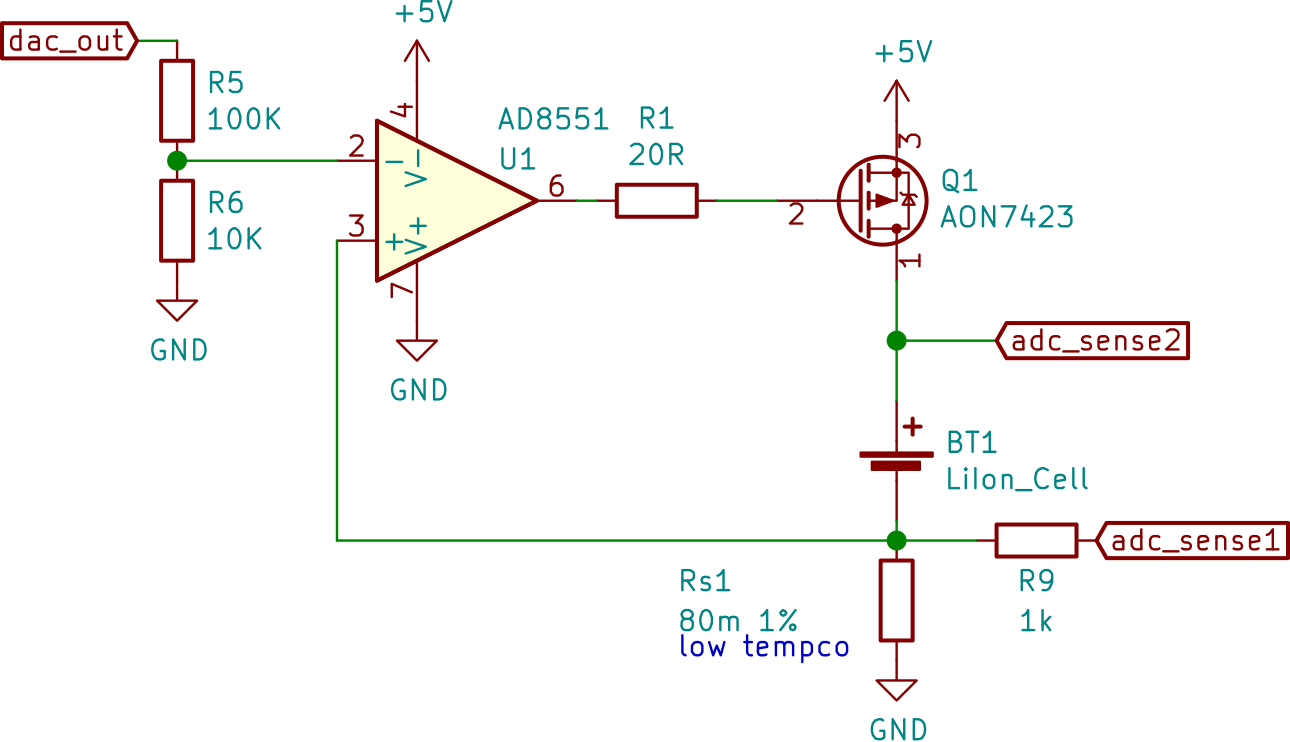
\includegraphics[]{img/CHARGING_LINE_SCHEMATIC.png}}
     \caption{Schemat części wykonawczej ładowarki. \label{img:charging_circuit}}
\end{figure}
Aby zachować w maksymalnym stopniu użyteczną rozdzielczość DAC, konieczne było dopasowanie poziomów napięć dzielnikiem napięcia.

\subsection{Element wykonawczy: tranzystor MOS typu P\label{section:mosfet} }
Wymagania jakie stawia dla MOSFETa taka struktura układu są następujące:
\begin{itemize}
    \item napięcie graniczne $U_{GS(th)} < 2.5\mathrm{V}$, pozwalające na całkowite otwarcie tranzystora przy rozładowanym ogniwie.
    \item niski opór otwarcia $R_{DS(on)}$, nie ograniczający prądu przy wystąpieniu dużej rezystancji wewnętrznej ogniwa.
    \item mały opór termiczny złącze-obudowa $R_{thJC}$, pozwalający na rozproszenie ciepła podczas pracy w trybie liniowym
\end{itemize}
Aby wybrać najlepiej działający tranzystor, projekt PCB przygotowano tak, aby można było wlutować tranzystory w 3 różnych standardach obudowy. Porównanie parametrów wybranych elementów znajduje się w tablicy \ref{tab:mosfets}.

\begin{table}[hbtp]
\caption{Parametry wybranych tranzystorów.\label{tab:mosfets}}
\centerline{\begin{tabular}{|c|c|c|c|c|}
\hline
nr. prod & $U_{GS(th)}$, mV & $R_{DS(on)}, \mathrm{m\Omega}$, & $R_{thJC}, \mathrm{\degree C/W}$ & obudowa \\
\hline
AON7407 & 550 & 18 & 3.5 & 8DFN 3x3 \\
\hline
AON7423 & 500 & 8.5 & 1.1 & 8DFN 3.3x3.3 \\ 
\hline
SIA427DJ-T1-GE3 & max 800 & 32 & 5.3 & PPak SC-70-6 \\
\hline
SI7615CDN-T1-GE3 & max 1000 & 20.3 & 2.9 & PPak 1212-8 \\
\hline
\end{tabular}}
\end{table}
Jak widać, AON7423 jest pod każdym względem lepszy i zostanie wybrany jako docelowy jeżeli nie wystąpią żadne nieprzewidziane czynniki.\remark{czas przyszły tutaj nie jest odpowiedni.}
\subsection{Regulator tranzystora: wzmacniacz operacyjny}
Ze względu na wybór tranzystora MOS, aby umożliwić kontrolę prądu prostymi algorytmami regulacji konieczne jest jego zlinearyzowanie. Zastosowanie pętli sprzężenia zwrotnego o dużym wzmocnieniu pozwoliło na zadawanie prąd za pomocą napięcia generowanego przez DAC mikrokontrolera, które to jest porównywane z napięciem na rezystorze pomiarowym. Dodatkowo takie rozwiązanie zapewniło eliminację wpływu temperatury tranzystora (która ulega znacznym wahaniom) oraz napięcia dren-źródło $U_{DS}$ (zależnego od stanu naładowania ogniwa) prąd wyjściowy. Taka konfiguracja ma jednak wadę: sprzężenie reaguje na prąd płynący przez rezystor $\mathrm{R_s}$, stąd przy małych wartościach tego prądu mogą wystąpić problemy z domknięciem tranzystora --- pewien niewielki prąd będzie cały czas doładowywał ogniwo, ale gdy zostanie on utrzymany na niskim poziomie, nie będzie miało to większego wpływu na działanie układu.

Aby zapewnić możliwość całkowitego otwarcia lub zamknięcie tranzystora, konieczne jest użycie wzmacniacza typu rail-to-rail na wyjściu. Dodatkowo, ze względu na wydzielane w układzie ciepło, wybrano wzmacniacz o bardzo niskim współczynniku cieplnym wejściowego napięcia niezrównoważenia ('zero drift'). Ponieważ dokładność działania zależy od wejściowego napięcia niezrównoważenia, zwrócono uwagę także aby ten parametr był utrzymany na niskim poziomie ('zero offset').

Wybrano wzmacniacz AD8551, który zapewnia 'input offset drift' nie większy niż $\mathrm{0.005 \mu V/\degree C}$ i bardzo niskie wejściowe napięcie niezrównoważenia $\mathrm{<1\mu V}$
\subsection{Element pomiarowy: rezystor}
Do pomiaru prądu płynącego przez ogniwo zastosowano rezystor o oporze $\mathrm{80m\Omega}$. Maksymalny spadek napięcia na elemencie pomiarowym, zapewniający poprawne działanie układy i odpowiednią dokładność pomiaru bez zbędnej komplikacji struktury przewidziany był na 250mV. Zastosowany opornik w przewidzianym zakresie użytkowania daje napięcie maksymalne $\mathrm{U_{rs(max)}=0.08\Omega 3\,A = 240\,mV}$. Wybór nieoptymalnej wartości jest spowodowany brakiem dostępności na rynku opornika o tej rezystancji i dokładności dokładności 1\%. Maksymalna moc wydzielana na oporniku wynosi $\mathrm{R_s*I_{cell(max)}^2 = 0.08 3^2 = 0.72\,W}$\remark{przy mocach maksymalnych dobrze uwzględniać możliwe błędy związane z pomiarem i regulacją, tzn. maksymalny prąd jest pewnie trochę większy jak 3~A, \ldots}\remark{zwykle symbole we wzorach pisze się normalną czcionką matematyczną, tzn. nie wszystko w mathrm, tylko jednoski.}, co maksymalnej dopuszczonej przez producenta mocy 3 W, konstrukcji opartej o pytkę ze specjalnego stopu, umieszczeniu w dużej odległości od źródeł ciepła i dobrym jego odprowadzaniu zapewnia minimalizację błędów wynikających ze zmian oporu wraz z temperaturą.
\subsection{Sterownik, regulator, zadajnik: mikrokontroler}
W rozważanym układzie przed mikrokontrolerem stawia się następujące zadania:
\begin{itemize}
    \item sterowanie następowaniem po sobie etapów procesu,
    \item regulacja prądu dostarczanego do ogniwa,
    \item zadawanie wartości tego prądu z użyciem przetwornika C/A\remark{wcześniej używał Pan DAC},
    \item pomiar napięcia na ogniwie,
    \item zapewnienie bezpieczeństwa procesu,
    \item obsługa przycisków i diód sygnalizacyjnych,
    \item komunikacja z komputerem.
\end{itemize}
W tym celu wybrano jednostkę ATtiny414, której istotne dla projektu parametry wyszczególniono poniżej, za \cite{tiny414datasheet}:
\begin{itemize}
    \item procesor: AVR RISC 8 bit, 20 MHz, sprzętowe mnożenie,
    \item pamięć: 4 kB program, 256 B SRAM,
    \item DAC: 8 bit, wewnętrzne napięcie odniesienia,
    \item ADC: 10 bit, akumulacja do 64 pomiarów, wewnętrzne napięcie odniesienia, 
    \item nap. odniesienia: 4.3, 2.5, 1.5, 1.1, 0.55 V,
    \item sprzętowe wsparcie UART,
    \item I/O: 12 programowalnych linii
\end{itemize}

\section{Projekt PCB}
Projekt płytki drukowanej, przedstawiony na rys. \ref{img:pcb_colored} został wykonany w darmowym środowisku KiCad. Wykonanie projektu przewidziano na laminacie dwustronnym o grubości miedzi 70 um.

\begin{figure}[hbtp]
     \resizebox{\linewidth}{!}{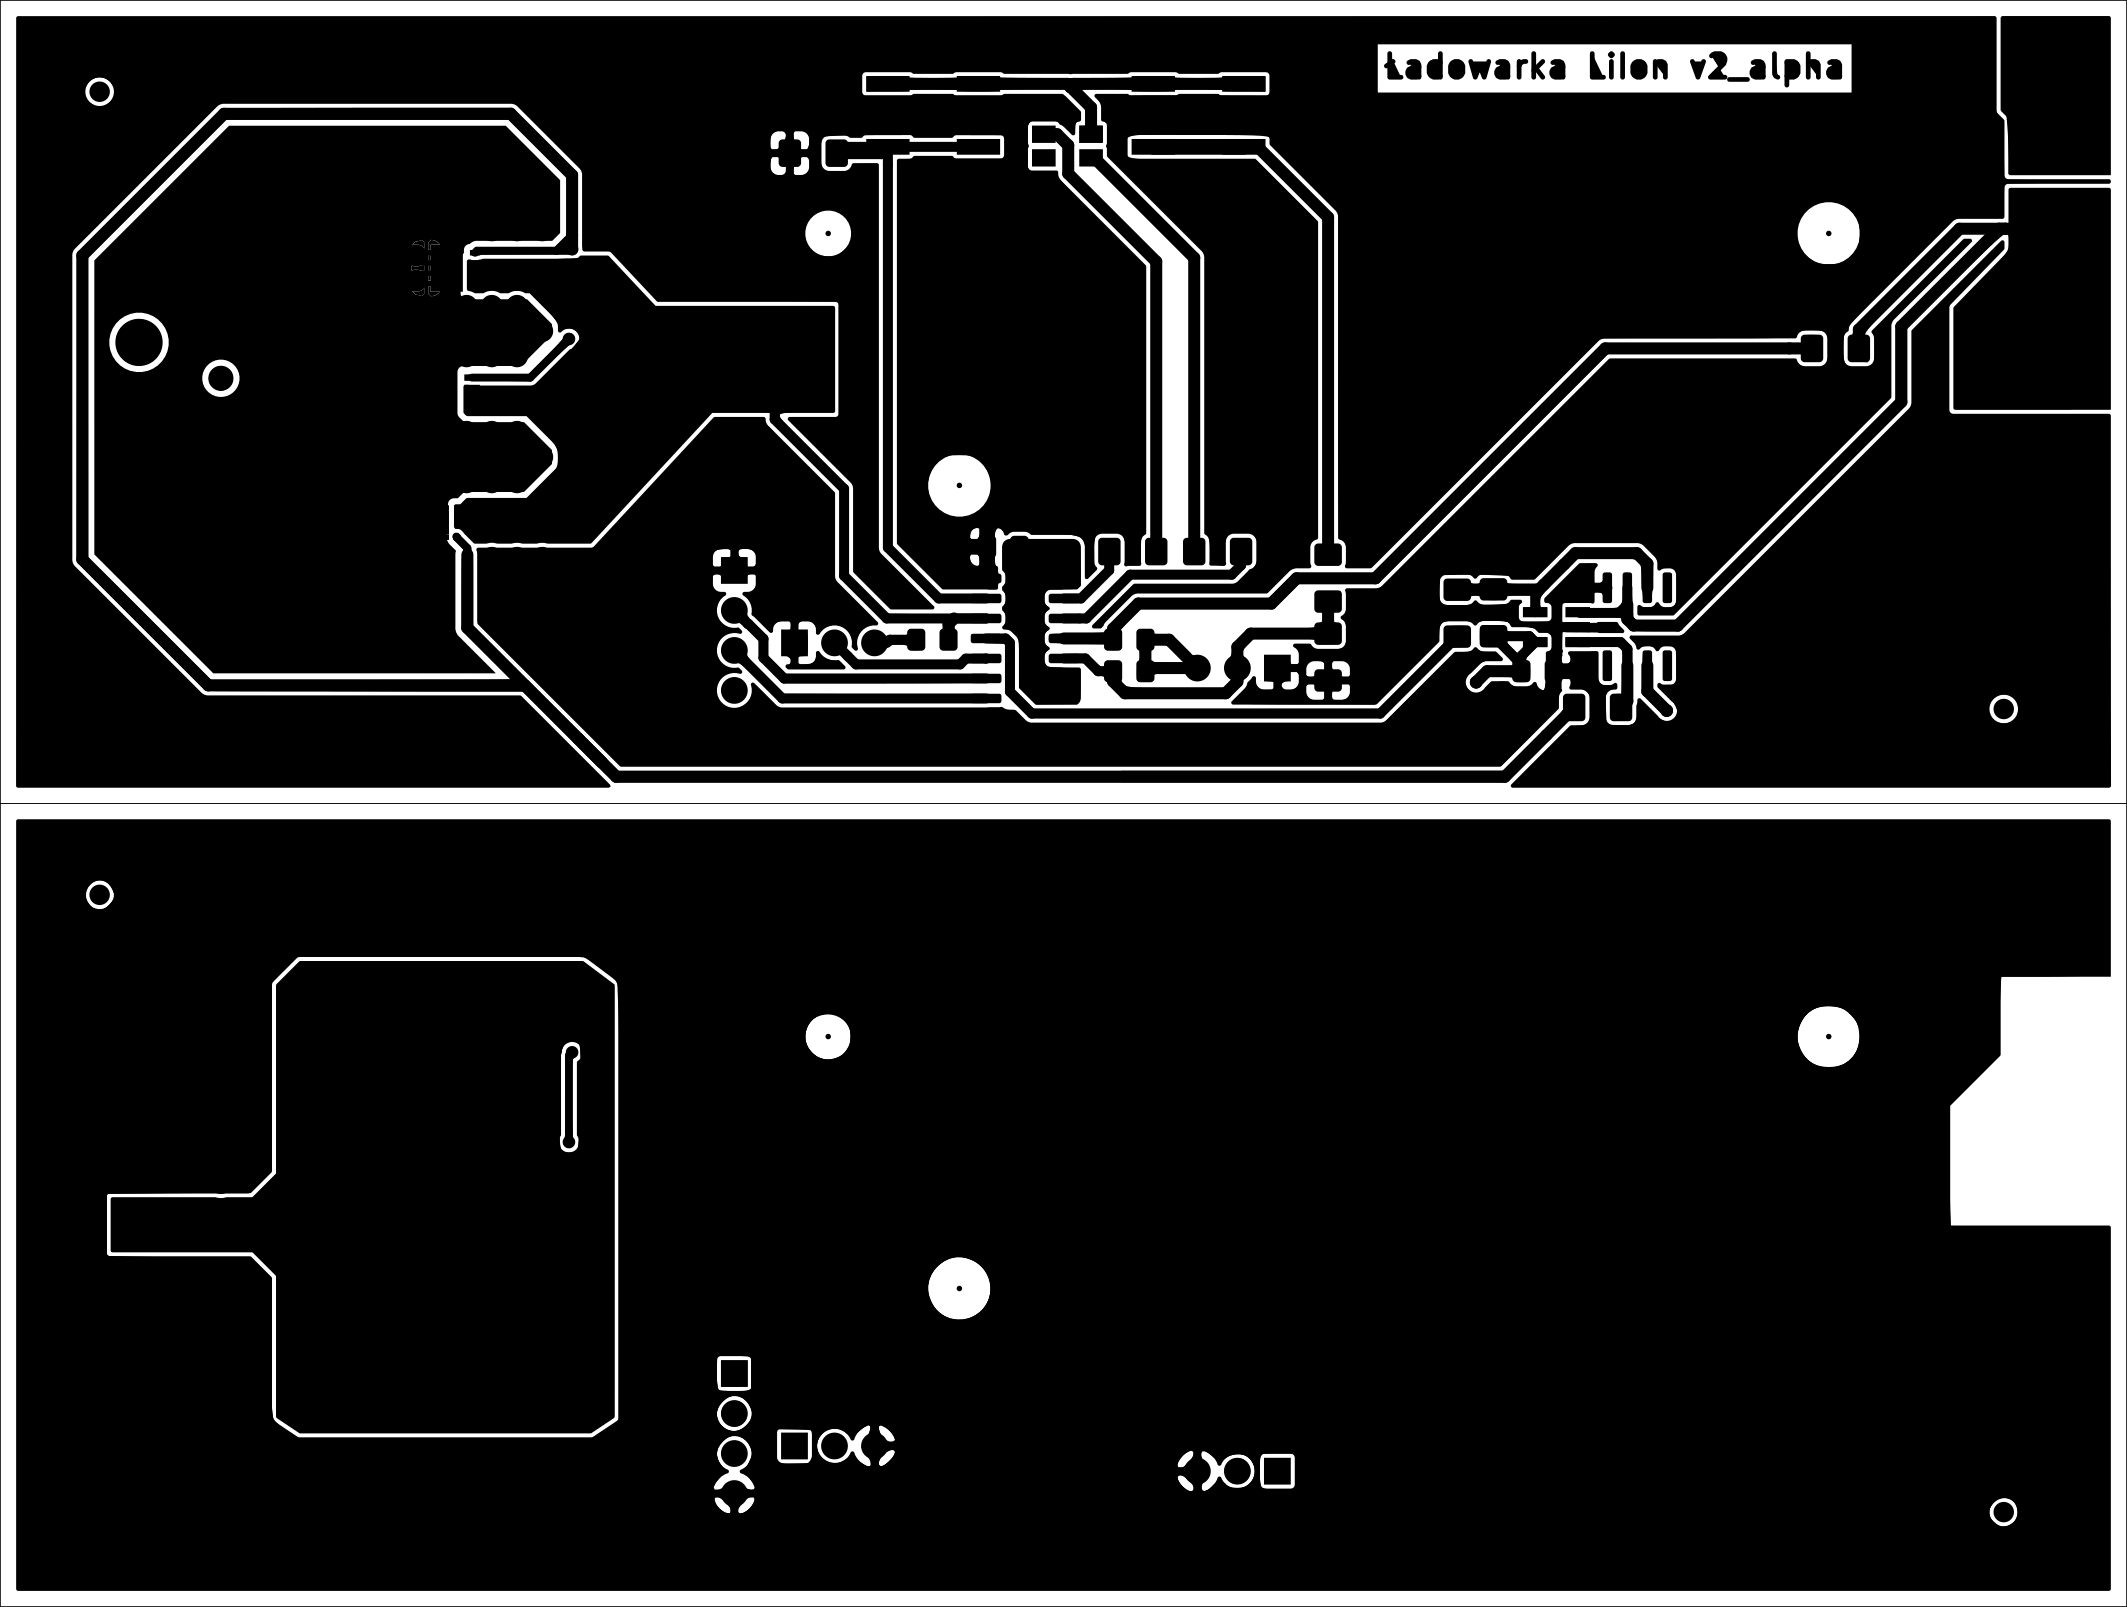
\includegraphics[]{img/plytka_bw.png}}
     \caption{Projekt PCB. \label{img:pcb_colored}}
\end{figure}

Aby zapewnić odporność na zakłócenia \remark{i emisję fal elektromagnetycznych}, na ile to możliwe zachowano ciągłość masy GND na spodniej powierzchni płytki. W tym samym celu rozlano +5 V na górnej powierzchni. 

Aby umożliwić przetestowanie kilku tranzystorów jak zaznaczono w punkcie \ref{section:mosfet}, przewidziane są pola na 3 różne standardy wyprowadzeń. Wokół niech znajdują się otwory, w których przewidziany jest montaż odcinków drutu 0.75 mm$^2$, pełniących rolę radiatora.

Rezystor pomiarowy znajduje się między ujemnym biegunem ogniwa i masą, maksymalnie oddalony od źródła ciepła jakim jest tranzystor. 

Sygnał z biegunów jest sprowadzony\remark{jakoś nie pasuje mi to słowo} do mikrokontrolera, alby mógł mierzyć napięcie na ogniwie, a napięcie na rezystorze pomiarowym względem wspólnej masy doprowadzone jest również do wzmacniacza operacyjnego. Aby zabezpieczyć się przed zakłóceniami pochodzącymi od układu próbkującego przetwornika A/C, sygnał z ujemnego bieguna jest doprowadzony do mikrokontrolera przez rezystor 1k i buforowany na miejscu kondensatorem 100nF. Kondensator znajduje się również przy doprowadzeniu sygnału z bieguna dodatniego, aby ograniczyć ewentualny wpływ impedancji linii.

Założono, że napięcie na rezystorze pomiarowym będzie nie większe niż 250mV, zatem sygnał do z przetwornika C/A musi zawierać się w tym samym przedziale. Aby w pełni wykorzystać rozdzielczość przetwornika, wybrano wewnętrzne napięcie odniesienia 2.5V, stąd najwyższe napięcie wyjściowe wyniesie 2.49 V. Aby dopasować je do napięć na elemencie pomiarowym, wykorzystano dzielnik napięcia złożony z rezystorów 10k i 91k\remark{na schemacie ma Pan 10k i 100k}. Napięcie maksymalne na wejściu wzmacniacza jest równe $2.49*10/(10+91) = 0.247$ V, czyli nieznacznie więcej niż przewidziane maksymalnie 0.24 V na rezystorze. Takie dopasowanie poziomów jest zadowalające.
\section{Weryfikacja projektu za pomocą symulacji SPICE}
Istotny fragment projektu został zamodelowany w programie LTSpice jak na rys. \ref{img:modelLTv1}
\begin{figure}[hbtp]
\centering
     \resizebox{0.8\linewidth}{!}{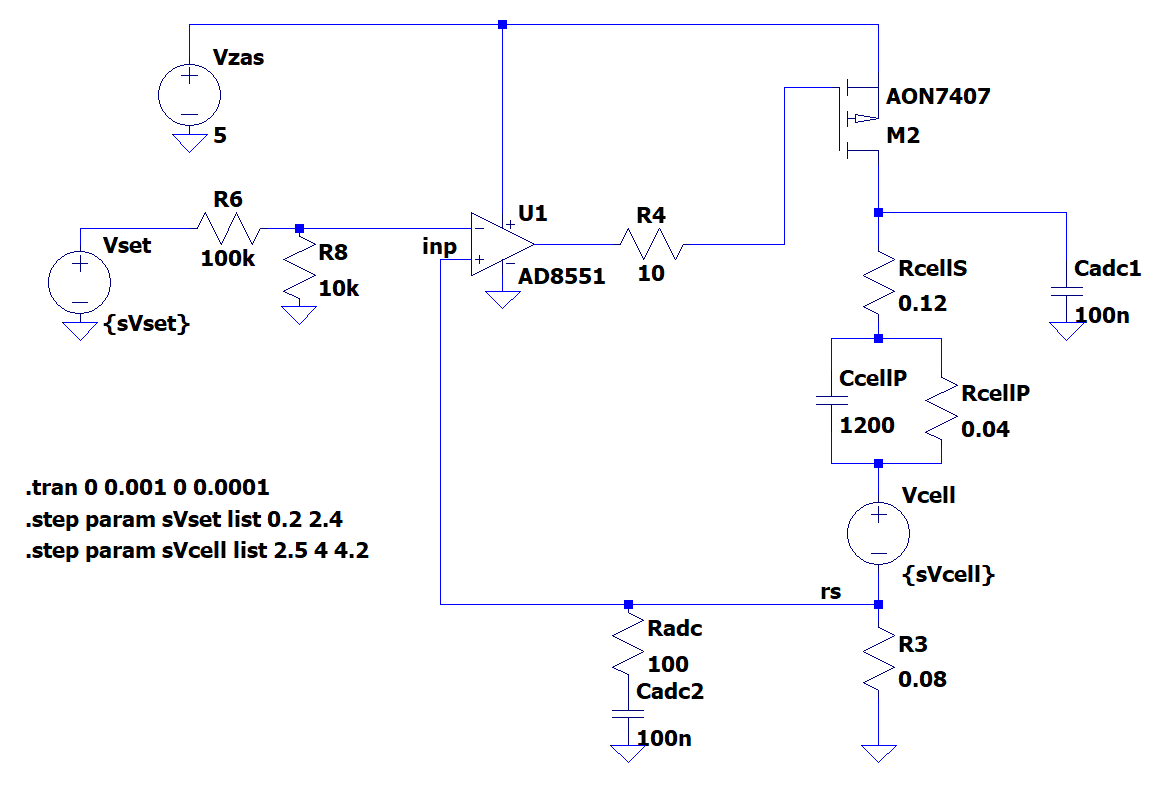
\includegraphics{img/odlschem.png}}
     \caption{Model w części wykonawczej w LTSpice. \label{img:modelLTv1}}
\end{figure}
Model ogniwa został przyjęty za \cite{8759769_cellmodel1storder}. W praktyce dla symulacji znaczenie ma tylko rezystancja szeregowa równa 120m$\Omega$ i napięcie na ogniwie.

Symulacja typu transient dla prądów 230 i 2730 mA przy napięciach na ogniwie 2.5, 4 i 4.2 V wykazała poprawne zachowanie układu, napięcia bez oscylacji osiągały zadane wartości.\remark{dobrze by umieścić te wyniki w pracy. Te charakterystyki Nyquista lub/i Bodego też.}

\chapter{Realizacja prototypu}
\section{Kolejność działania i bieżąca modyfikacja projektu\label{section:przerobki}}
Płytka drukowana została wykonana metodą termotransferu. Z powodu braku soldermaski projekt realizowany jest etapami, aby zweryfikować poprawność montażu. Kolejność działań jest następująca:
\begin{enumerate}
    \item Weryfikacja i ewentualna naprawa ścieżek.
    \item Montaż mikrokontrolera wraz z koniecznymi elementami pasywnymi i sprawdzenie działania linii programowania.
    \item Montaż elementów pasywnych, diód sygnalizacyjnych i przycisków.
    \item Weryfikacja działania linii komunikacyjnych.
    \item Weryfikacja działaniu pomiaru napięcia ogniwa oraz przetwornika C/A.
    \item Montaż i sprawdzenie działania wzmacniacza.
    \item Montaż i sprawdzenie działania tranzystora.
    \item Budowa obciążenia testowego i pierwsze testy działania z docelowym rezystorem.
    \item Kalibracja przetwornika A/C.
    \item Montaż uchwytu ogniwa i testy na ogniwie.
\end{enumerate}
Po wytrawieniu w skutek defektu warstwy zabezpieczającej ścieżka doprowadzająca sygnał z dodatniego bieguna ogniwa została rozpuszczona powodując przerwę około 1mm, co zostało naprawione mostkiem z drutu.

Nowa seria mikrokontrolerów ATtiny (produkowana przez Microchip po przejęciu Atmel), do której należy wybrana jednostka, aby zwiększyć liczbę możliwych do wykorzystania pinów, jest programowana przez interfejs UPDI, który pozwala na komunikację half-duplex po jednym linii, pomijając połączenie masy. Aby nie kupować drogiego programatora producenta, wykorzystano rozwiązanie pozwalające na programowanie z użyciem zwykłego adaptera USB-TTL i rezystora\cite{pyupdi}.
\begin{figure}[hbtp]
\centering
     \resizebox{0.8\linewidth}{!}{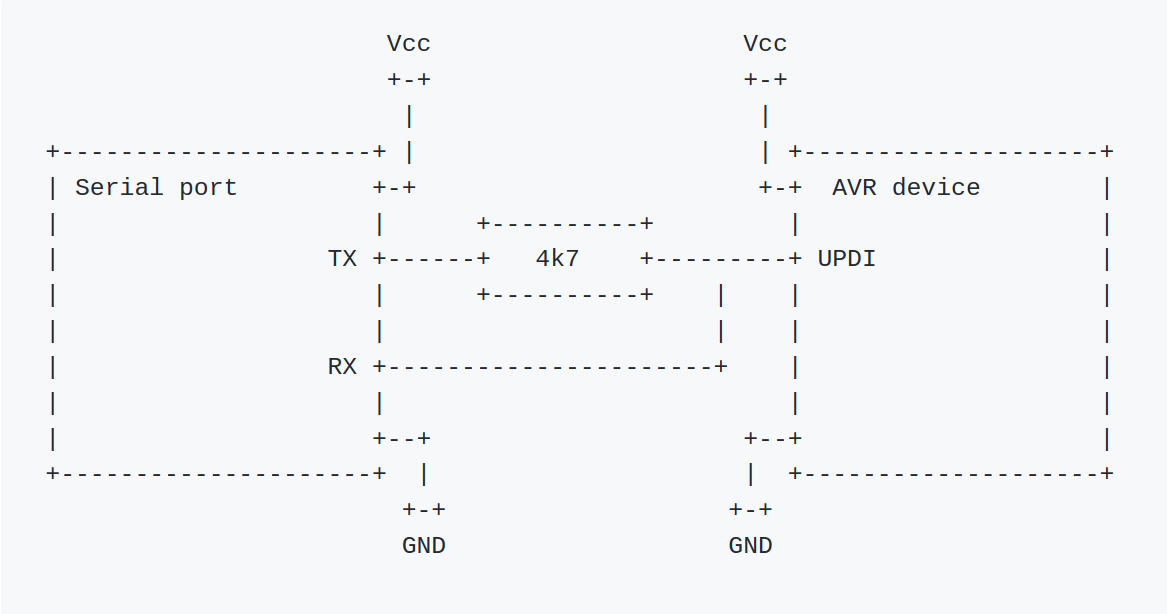
\includegraphics[]{img/pyupdi.png}}
     \caption{Podłączenie programatora, wykorzystano grafikę z \cite{pyupdi}\label{img:pyupdi}}
\end{figure}
Producent zaleca podłączenie kondensatora chroniącego przed zakłóceniami pomiędzy pin resetu a masę, jednocześnie ostrzegając, że dla niektórych innych interfejsów może uniemożliwić to ich funkcjonowanie\cite{avr_hardware}. Jak sprawdzono, konieczne było wylutowanie kondensatora także w przypadku UPDI.

Podczas montażu diód sygnalizacyjnych okazało się, że użyty footprint jest przeznaczony dla elementu ze wspólną katodą, a zakupiony komponent miał niezależne katody, położone na innych pinach. Obrócenie i włączanie zwieraniem do masy zamiast do zasilania umożliwiło zachowanie PCB.

Podczas weryfikacji działania przetworników stwierdzono, że układ C/A działa jak zakładano, a układ A/C zaniża mierzone napięcie o około 0.5V. Błąd ten był stały w mierzonych przedziałach, więc odpowiednia kalibracja, przeprowadzona w późniejszych etapach pozwoliła go wyeliminować.\remark{0.5V? dobrze by było ustalić dlaczego. C/A na obu wejściach ma te kondensatory 100nF? Napięcie referencyjne jest na pewno właściwe?}

Podczas weryfikacji poprawności działania wzmacniaczy stwierdzono, że przyczyną ich zapłonu jest błędne podłączenie zasilania i masy. Na obydwu footprintach wyłącznie te piny były zamienione. Przecięcie 2 ścieżek i dodanie 3 rezystorów 0~$\Omega$ pozwoliło w czysty sposób naprawić pomyłkę, bez wpływu na jakość działania układu.

Po zamontowaniu tranzystora stwierdzono, że w skutek pomyłki przy rysowaniu schematu, symbol tranzystora był odwrócony (w tym układzie jest użyty odwrotnie niż w większości zastosowań), a co za tym idzie, dren ze źródłem był odwrócony. Po wykryciu, że powodem przepływu prądu i pewnego spadku napięcia jest wewnętrzna dioda, i odwróceniu elementu układa działa poprawnie. Konieczna była rekonfiguracja obszaru odprowadzania ciepła i przeniesienie rezystora spod wzmacniacza, aby doprowadzał sygnał do ścieżki bramki. Wykorzystano zakupiony radiator z blachy miedzianej 0.6mm przeznaczony dla obudów D2Pak o deklarowanym oporze cieplnym do otoczenia równym $\mathrm{11\degree \,C/W}$ przy naturalnej konwekcji. 

Ponieważ podanie zbyt dużego napięcia na ogniwo lub zwarcie biegunów może prowadzić do zniszczenia ogniwa a nawet zapalenia się, aby bezpiecznie sprawdzić działanie układu wykonano obciążenie testowe z diód o odpowiedniej mocy, którego schemat przedstawiono na rys. \ref{img:testload}. Urządzenie to pozwala także na bezpieczne rozładowanie ogniw do około 2.5 V.
Aby ułatwić testy, zgodnie z metodą 'hardware-in-the-loop', cały proces nadzoruje skrypt w środowisku MATLAB, a mikroprocesor zajmuje się wymianą danych między peryferiami a komputerem.
\begin{figure}[hbtp]
    \centering
    \resizebox{0.5\linewidth}{!}{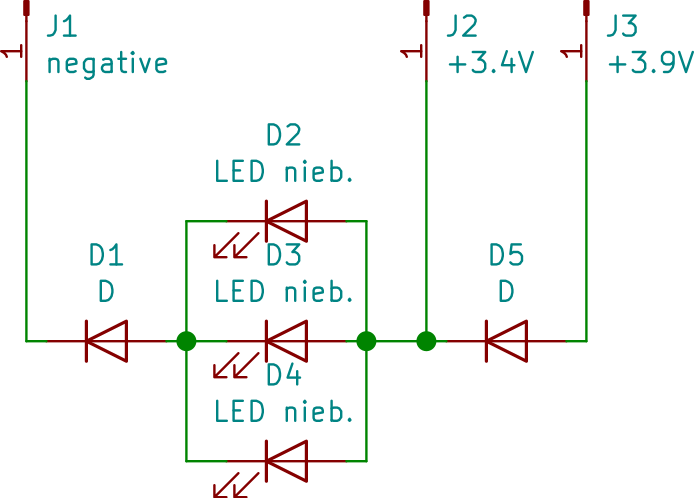
\includegraphics[]{img/testload.png}}
    \caption{Schemat obciążenia testowego. \label{img:testload}}
\end{figure}

Wykorzystując fakt, że napięcie przewodzenia diód zmienia się w zależności od prądu, wykonano pomiary przez przetwornik A/C i niezależny woltomierz, tak aby skalibrować przetwornik. Zebrano dane dla obu stron ogniwa, i dla osiągnięcia większej dokładności skalibrowano je niezależnie.
\begin{figure}[hbtp]
     \resizebox{\linewidth}{!}{fity pomiarów ADC tu}
     \caption{Kalibracja przetwornika A/C \label{img:ADCfitting}}
\end{figure}
Dzięki temu odwzorowano pomiary woltomierzem z dokładnością do 0.01 V.

Testy wykonane na docelowych ogniwach przebiegły pomyślnie. Ze względu na dużą rezystancje wewnętrzną głęboko rozładowanych ogniw, moc wydzielana na tranzystorze nigdy nie osiąga zakładanej wartości. Temperatura na tranzystorze nie przekracza maksymalnie dopuszczalnej.

\section{Stan finalny części sprzętowej}
Ostatecznie projekt wykonany jest na bazie płytki PCB z oryginalnego projektu z modyfikacjami z punktu \ref{section:przerobki}. Sprawdzono z pozytywnym wynikiem stabilność funkcjonowania dla prądu 2A i napięcia początkowego ogniwa 2.5 V, co przekłada się na około 3.7 W mocy wydzielanej na tranzystorze. Na testy większych obciążeń nie pozwalają posiadane ogniwa.

\section{Implementacja potrzebnych funkcjonalności}
Ze względu na fakt, że przeznaczeniem urządzenia są zadania eksperymentalne, które zawsze zakładają zbieranie danych na komputerze, zdecydowano o implementacji całej funkcjonalności za pomocą skryptów w środowisku MATLAB. Pozwala to także na bieżącą obserwację parametrów procesu.

Zaimplementowane funkcjonalności pozwalają na ciągłe monitorowanie napięcia na ogniwie oraz realizacje protokołu ładowania CC-CV do zadanych wartości napięcia oraz prądu maksymalnego i granicznego końcowego.

Skrypt ładujący CC-CV działa następująco:
\begin{enumerate}
    \item Sprawdzane są napięcia na stykach uchwytu. Jeżeli nie mieszczą się w założonym przedziale, ładowanie jest wyłączane i użytkownik jest informowany o błędzie.
    \item Gdy użytkownik potwierdzi parametry ładowania, urządzenie utrzymuje stały prąd do momentu osiągnięcia napięcia docelowego.
    \item Po osiągnięciu napięcia będącego rożnym od docelowego o pewien ustalony próg zadziałania (np. -0.03 V), poziom ustalony przed rozpoczęciem jest utrzymywany przez regulator PI. 
    \item Po osiągnięciu wartości prądu poniżej progu końcowego lub wystąpieniu błędu, ładowanie jest wyłączane, a użytkownik powiadamiany o rezultacie.
\end{enumerate}


\chapter{Testy i weryfikacja}

Ponieważ rezystancja wewnętrzna ogniwa ulega w procesie ciągłym zmianom, co więcej, szybkość tych zmian także nie jest stała, stąd jakość regulacji może być zdecydowanie polepszona użyciem takich technik jak np. gain scheduling.
Mimo, że układ jest statyczny względem zadanego prądu, odpowiednio duże wzmocnienie regulatora PI zapewnia akceptowalne mały uchyb w całym czasie regulacji\remark{tego trochę nie rozumiem. Ma Pan regulator P prądu, o dużym wzmocnieniu. I ten uchyb jest mały, regulator PI nic tutaj nie zmienia. Tyle, że ma Pan regulowane napięcie bez uchybu w stanie ustalonym, a prąd z drobnym uchybem.}. 
Wykorzystanie przetwornika A/C na ujemnym biegunie ogniwa nie pozwala na dokładne pomiary wartości prądu, ale daje podgląd dynamiki jego zmian. Przebieg napięć i prądów dla procesu przy wstępnych nastawach przedstawiono na rys. dla ładowania ogniwa o pojemności nominalnej 2700 mAh prądem 1.9 A do napięcia 4.0 V kończąc ładowanie przy prądzie 1000 mA.
\begin{figure}[hbtp]
     \resizebox{\linewidth}{!}{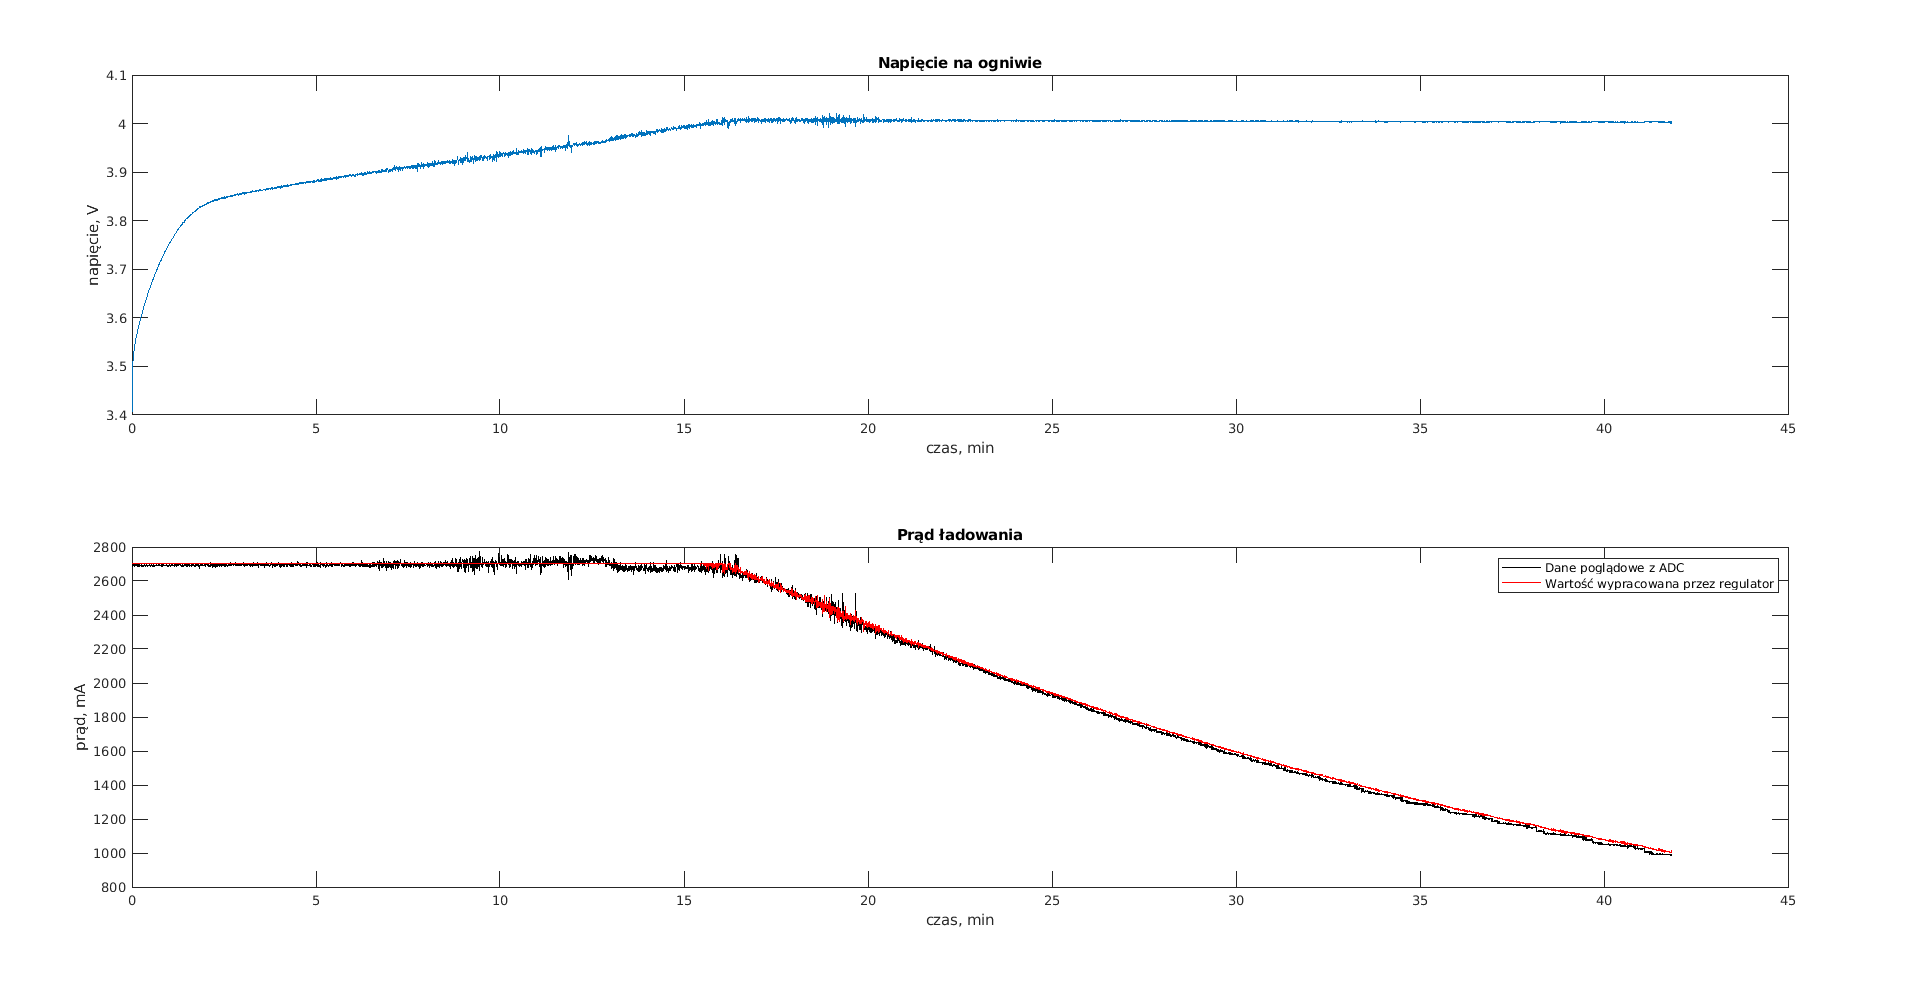
\includegraphics[]{img/bezkondensatorze.png}}
     \caption{Pierwszy test. \label{img:1strun}}
\end{figure}
W miarę zbliżania się do napięcia 4 V, między 5. a 21. minutą, można zaobserwować narastające szumy na napięciu ogniwa. Są one mieszczą się one zazwyczaj w zakładanej tolerancji dla napięcia ładowania, ale ich szybkozmienny charakter sugeruje występowanie w układzie oscylacji. Jako że sygnał z przetwornika jest uśrednieniem 64 kolejnych pomiarów, oscylacje muszą być bardzo znaczące.
Najbardziej prawdopodobnym ich źródłem, jako, że objawiają się przede wszystkim wahaniami prądu, jest wadliwy projekt sprzężenia zwrotnego od rezystora pomiarowego do tranzystora. Za pomocą symulacji SPICE zweryfikowano zapas fazy układu dla zestawu parametrów, dla którego wystąpiły największe oscylacje.
\begin{figure}[hbtp]
     \resizebox{\linewidth}{!}{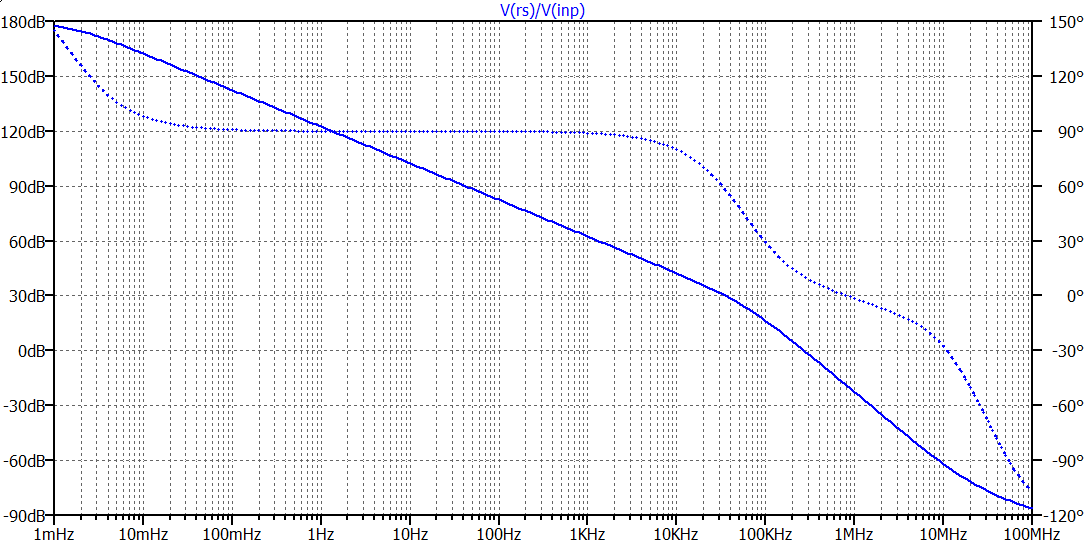
\includegraphics[]{img/bode_nocap.png}}
     \caption{Analiza małosygnałowa dla układu oscylującego: wykres Bodego \label{img:1strun}}
\end{figure}
W rezultacie stwierdzono, że zapas fazy wynosi około 10\degree. Teoretycznie układ powinien być stabilny dla każdego zapasu fazy > 0\degree, ale w praktyce wiele nieprzewidzianych czynników może doprowadzić do jego obniżenia, na przykład pojemność ścieżki pomiędzy wzmacniaczem a bramką tranzystora (która sama w sobie tworzy kondensator). W praktyce przyjmuje się że zapas fazy powinien wynosić 45\degree \cite{PhaseMargin_TERRELL1996383}.

Celem zwiększenia zapasu fazy poprzez do akceptowalnych wartości dodano kondensator pomiędzy wejście odwracające a wyjście wzmacniacza (rys. \ref{img:HereYouAreMrCap}), co zwiększyło zapas fazy do 45\degree (rys. \ref{img:MrBodeWithCap}).
\begin{figure}[hbtp]
    \centering
     \resizebox{0.7\linewidth}{!}{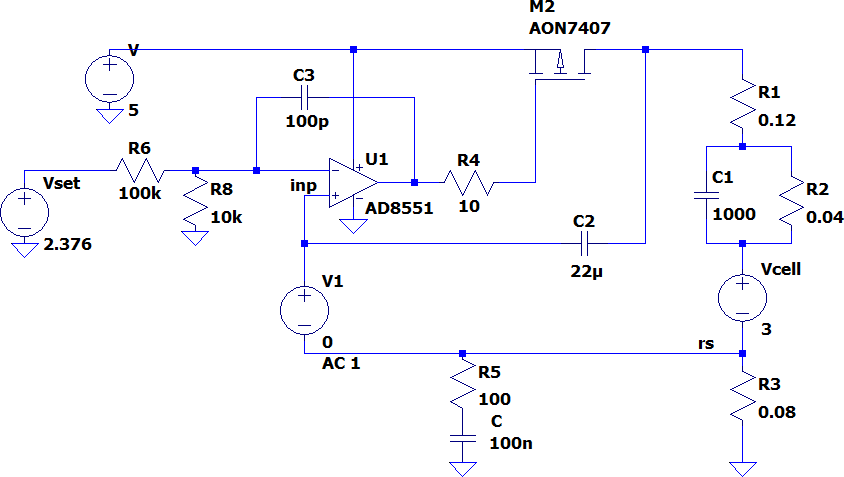
\includegraphics[]{img/how_cap_was_added.png}}
     \caption{Schemat układu lepiej tłumiącego drgania. \label{img:HereYouAreMrCap}}
\end{figure}
\begin{figure}[hbtp]
     \resizebox{\linewidth}{!}{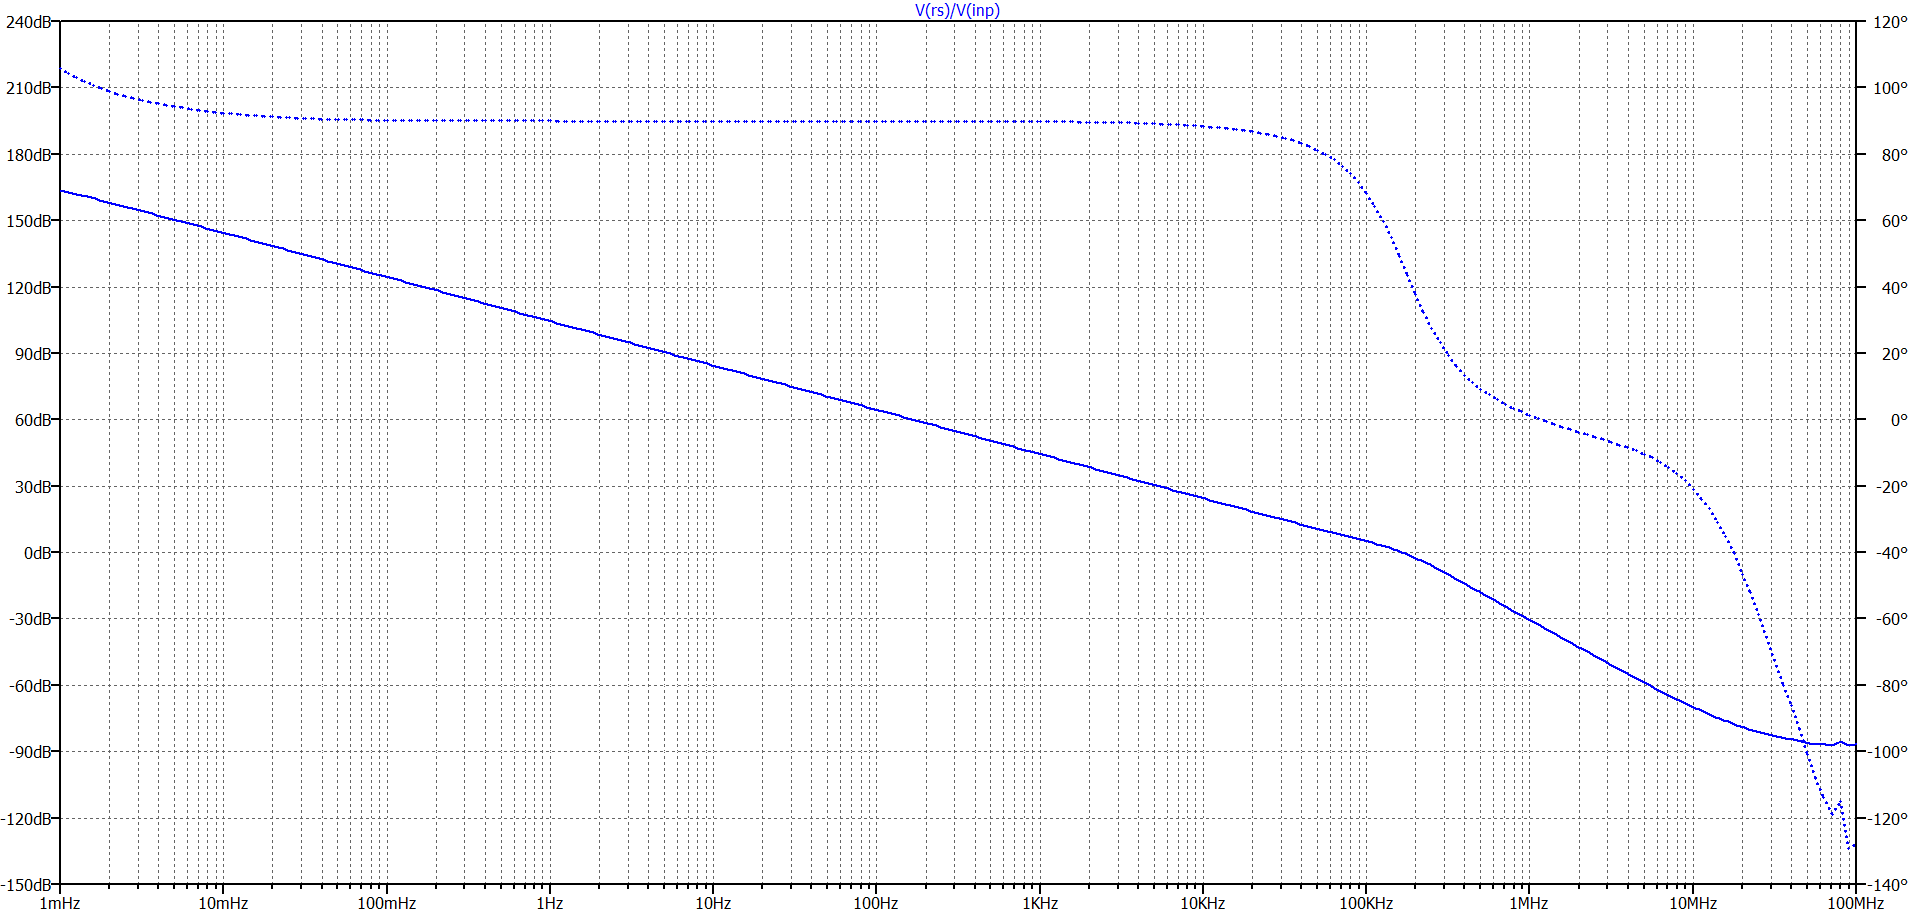
\includegraphics[]{img/bode_withcap.png}}
     \caption{Badanie zapasu fazy dla po dodaniu kompensatora. \label{img:MrBodeWithCap}}
\end{figure}

Po zastosowanych zmianach:
\begin{figure}[hbtp]
     \resizebox{\linewidth}{!}{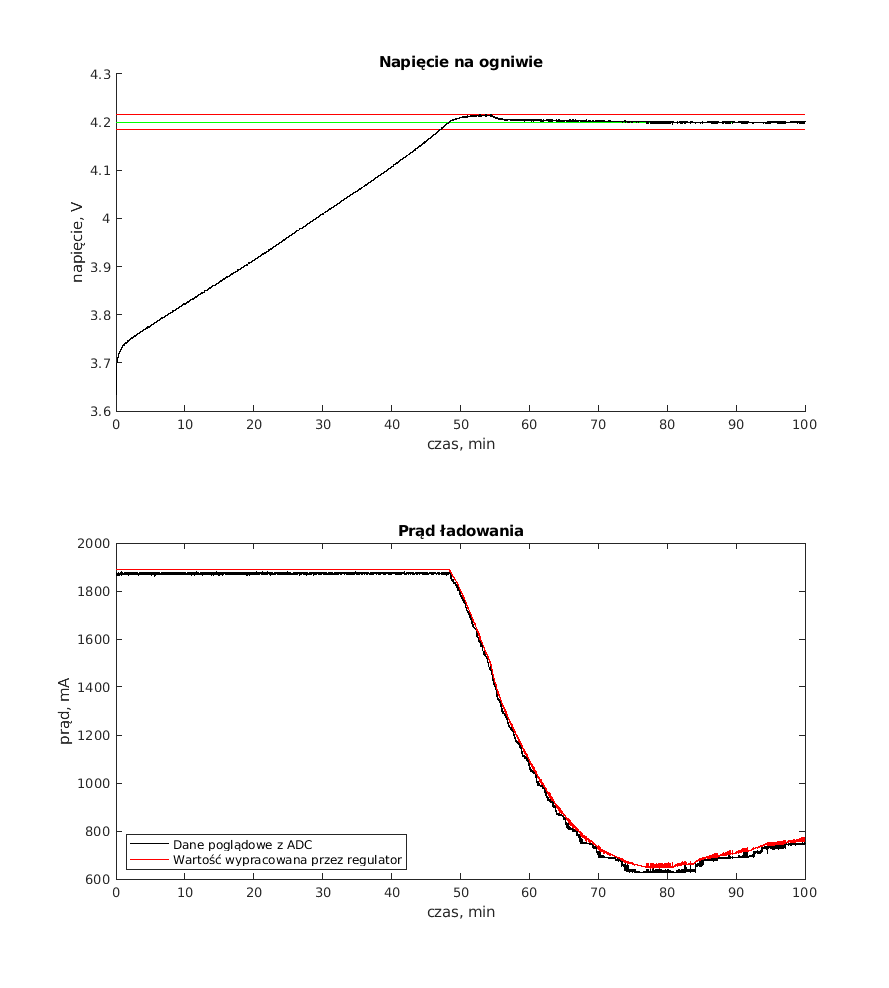
\includegraphics{img/prettyChargingAaaaandFailure.png}}
     \caption{Przebieg procesu ładowania. Widoczne uszkodzenie ogniwa. \label{img:PrettyChargeWithCellFailure}}
\end{figure}

\chapter{Uwagi końcowe}
Cele postawione w projekcie zostały z sukcesem zrealizowane. Urządzenie jest w stanie regulować prąd i napięcie ładowania, realizując założone strategie ładowania z przewidzianą dokładnością. Proces realizacji urządzenia ujawnił wiele błędów etapu projektowego, które jednak udało się naprawić bez wpływu na skuteczność działania ładowarki. Wykorzystanie wstępnie uruchomionego urządzenia pozwoliło na zebranie danych potrzebnych do określenia modelu, pozwalającego na dalsza poprawę działania. Skuteczność funkcjonowania udowadnia stosowny wykres zapisanego przebiegu procesu.

Zaprojektowane urządzenia z powodzeniem jest wykorzystywane przez autora na co dzień, demonstrując zaskakującą żywotność w warunkach eksploatacji na granicy możliwości.

\remark{to wypadało by jeszcze trochę rozszerzyć}

\bibliographystyle{unsrt} 
\bibliography{bibiking}

\end{document}
